% Options for packages loaded elsewhere
\PassOptionsToPackage{unicode}{hyperref}
\PassOptionsToPackage{hyphens}{url}
\documentclass[
  12pt,
  oneside]{book}
\usepackage{xcolor}
\usepackage[margin=2.5cm]{geometry}
\usepackage{amsmath,amssymb}
\setcounter{secnumdepth}{5}
\usepackage{iftex}
\ifPDFTeX
  \usepackage[T1]{fontenc}
  \usepackage[utf8]{inputenc}
  \usepackage{textcomp} % provide euro and other symbols
\else % if luatex or xetex
  \usepackage{unicode-math} % this also loads fontspec
  \defaultfontfeatures{Scale=MatchLowercase}
  \defaultfontfeatures[\rmfamily]{Ligatures=TeX,Scale=1}
\fi
\usepackage{lmodern}
\ifPDFTeX\else
  % xetex/luatex font selection
\fi
% Use upquote if available, for straight quotes in verbatim environments
\IfFileExists{upquote.sty}{\usepackage{upquote}}{}
\IfFileExists{microtype.sty}{% use microtype if available
  \usepackage[]{microtype}
  \UseMicrotypeSet[protrusion]{basicmath} % disable protrusion for tt fonts
}{}
\makeatletter
\@ifundefined{KOMAClassName}{% if non-KOMA class
  \IfFileExists{parskip.sty}{%
    \usepackage{parskip}
  }{% else
    \setlength{\parindent}{0pt}
    \setlength{\parskip}{6pt plus 2pt minus 1pt}}
}{% if KOMA class
  \KOMAoptions{parskip=half}}
\makeatother
\usepackage{color}
\usepackage{fancyvrb}
\newcommand{\VerbBar}{|}
\newcommand{\VERB}{\Verb[commandchars=\\\{\}]}
\DefineVerbatimEnvironment{Highlighting}{Verbatim}{commandchars=\\\{\}}
% Add ',fontsize=\small' for more characters per line
\usepackage{framed}
\definecolor{shadecolor}{RGB}{248,248,248}
\newenvironment{Shaded}{\begin{snugshade}}{\end{snugshade}}
\newcommand{\AlertTok}[1]{\textcolor[rgb]{0.94,0.16,0.16}{#1}}
\newcommand{\AnnotationTok}[1]{\textcolor[rgb]{0.56,0.35,0.01}{\textbf{\textit{#1}}}}
\newcommand{\AttributeTok}[1]{\textcolor[rgb]{0.13,0.29,0.53}{#1}}
\newcommand{\BaseNTok}[1]{\textcolor[rgb]{0.00,0.00,0.81}{#1}}
\newcommand{\BuiltInTok}[1]{#1}
\newcommand{\CharTok}[1]{\textcolor[rgb]{0.31,0.60,0.02}{#1}}
\newcommand{\CommentTok}[1]{\textcolor[rgb]{0.56,0.35,0.01}{\textit{#1}}}
\newcommand{\CommentVarTok}[1]{\textcolor[rgb]{0.56,0.35,0.01}{\textbf{\textit{#1}}}}
\newcommand{\ConstantTok}[1]{\textcolor[rgb]{0.56,0.35,0.01}{#1}}
\newcommand{\ControlFlowTok}[1]{\textcolor[rgb]{0.13,0.29,0.53}{\textbf{#1}}}
\newcommand{\DataTypeTok}[1]{\textcolor[rgb]{0.13,0.29,0.53}{#1}}
\newcommand{\DecValTok}[1]{\textcolor[rgb]{0.00,0.00,0.81}{#1}}
\newcommand{\DocumentationTok}[1]{\textcolor[rgb]{0.56,0.35,0.01}{\textbf{\textit{#1}}}}
\newcommand{\ErrorTok}[1]{\textcolor[rgb]{0.64,0.00,0.00}{\textbf{#1}}}
\newcommand{\ExtensionTok}[1]{#1}
\newcommand{\FloatTok}[1]{\textcolor[rgb]{0.00,0.00,0.81}{#1}}
\newcommand{\FunctionTok}[1]{\textcolor[rgb]{0.13,0.29,0.53}{\textbf{#1}}}
\newcommand{\ImportTok}[1]{#1}
\newcommand{\InformationTok}[1]{\textcolor[rgb]{0.56,0.35,0.01}{\textbf{\textit{#1}}}}
\newcommand{\KeywordTok}[1]{\textcolor[rgb]{0.13,0.29,0.53}{\textbf{#1}}}
\newcommand{\NormalTok}[1]{#1}
\newcommand{\OperatorTok}[1]{\textcolor[rgb]{0.81,0.36,0.00}{\textbf{#1}}}
\newcommand{\OtherTok}[1]{\textcolor[rgb]{0.56,0.35,0.01}{#1}}
\newcommand{\PreprocessorTok}[1]{\textcolor[rgb]{0.56,0.35,0.01}{\textit{#1}}}
\newcommand{\RegionMarkerTok}[1]{#1}
\newcommand{\SpecialCharTok}[1]{\textcolor[rgb]{0.81,0.36,0.00}{\textbf{#1}}}
\newcommand{\SpecialStringTok}[1]{\textcolor[rgb]{0.31,0.60,0.02}{#1}}
\newcommand{\StringTok}[1]{\textcolor[rgb]{0.31,0.60,0.02}{#1}}
\newcommand{\VariableTok}[1]{\textcolor[rgb]{0.00,0.00,0.00}{#1}}
\newcommand{\VerbatimStringTok}[1]{\textcolor[rgb]{0.31,0.60,0.02}{#1}}
\newcommand{\WarningTok}[1]{\textcolor[rgb]{0.56,0.35,0.01}{\textbf{\textit{#1}}}}
\usepackage{longtable,booktabs,array}
\usepackage{calc} % for calculating minipage widths
% Correct order of tables after \paragraph or \subparagraph
\usepackage{etoolbox}
\makeatletter
\patchcmd\longtable{\par}{\if@noskipsec\mbox{}\fi\par}{}{}
\makeatother
% Allow footnotes in longtable head/foot
\IfFileExists{footnotehyper.sty}{\usepackage{footnotehyper}}{\usepackage{footnote}}
\makesavenoteenv{longtable}
\usepackage{graphicx}
\makeatletter
\newsavebox\pandoc@box
\newcommand*\pandocbounded[1]{% scales image to fit in text height/width
  \sbox\pandoc@box{#1}%
  \Gscale@div\@tempa{\textheight}{\dimexpr\ht\pandoc@box+\dp\pandoc@box\relax}%
  \Gscale@div\@tempb{\linewidth}{\wd\pandoc@box}%
  \ifdim\@tempb\p@<\@tempa\p@\let\@tempa\@tempb\fi% select the smaller of both
  \ifdim\@tempa\p@<\p@\scalebox{\@tempa}{\usebox\pandoc@box}%
  \else\usebox{\pandoc@box}%
  \fi%
}
% Set default figure placement to htbp
\def\fps@figure{htbp}
\makeatother
% definitions for citeproc citations
\NewDocumentCommand\citeproctext{}{}
\NewDocumentCommand\citeproc{mm}{%
  \begingroup\def\citeproctext{#2}\cite{#1}\endgroup}
\makeatletter
 % allow citations to break across lines
 \let\@cite@ofmt\@firstofone
 % avoid brackets around text for \cite:
 \def\@biblabel#1{}
 \def\@cite#1#2{{#1\if@tempswa , #2\fi}}
\makeatother
\newlength{\cslhangindent}
\setlength{\cslhangindent}{1.5em}
\newlength{\csllabelwidth}
\setlength{\csllabelwidth}{3em}
\newenvironment{CSLReferences}[2] % #1 hanging-indent, #2 entry-spacing
 {\begin{list}{}{%
  \setlength{\itemindent}{0pt}
  \setlength{\leftmargin}{0pt}
  \setlength{\parsep}{0pt}
  % turn on hanging indent if param 1 is 1
  \ifodd #1
   \setlength{\leftmargin}{\cslhangindent}
   \setlength{\itemindent}{-1\cslhangindent}
  \fi
  % set entry spacing
  \setlength{\itemsep}{#2\baselineskip}}}
 {\end{list}}
\usepackage{calc}
\newcommand{\CSLBlock}[1]{\hfill\break\parbox[t]{\linewidth}{\strut\ignorespaces#1\strut}}
\newcommand{\CSLLeftMargin}[1]{\parbox[t]{\csllabelwidth}{\strut#1\strut}}
\newcommand{\CSLRightInline}[1]{\parbox[t]{\linewidth - \csllabelwidth}{\strut#1\strut}}
\newcommand{\CSLIndent}[1]{\hspace{\cslhangindent}#1}
\setlength{\emergencystretch}{3em} % prevent overfull lines
\providecommand{\tightlist}{%
  \setlength{\itemsep}{0pt}\setlength{\parskip}{0pt}}
\usepackage{float}
\usepackage{booktabs}
\usepackage{longtable}
\usepackage{array}
\usepackage{multirow}
\usepackage{wrapfig}
\usepackage{colortbl}
\usepackage{pdflscape}
\usepackage{tabu}
\usepackage{threeparttable}
\usepackage{threeparttablex}
\usepackage[normalem]{ulem}
\usepackage{makecell}
\usepackage{xcolor}
\usepackage{bookmark}
\IfFileExists{xurl.sty}{\usepackage{xurl}}{} % add URL line breaks if available
\urlstyle{same}
\hypersetup{
  pdftitle={xtitle: coherence \& propositions observations in :schizophrenia: threads},
  pdfauthor={st. schwarz},
  hidelinks,
  pdfcreator={LaTeX via pandoc}}

\title{xtitle: coherence \& propositions observations in :schizophrenia: threads}
\author{st. schwarz}
\date{2025-10-15}

\begin{document}
\maketitle

{
\setcounter{tocdepth}{1}
\tableofcontents
}
\chapter{index}\label{index}

Hausarbeit im Seminar: \emph{Sprache und Psychose (PHILGEIST\_S\_16827\_25S)}\\
Dozent: Anatol Stefanowitsch\\
abgegeben von: placeholder\\
MtrNr: placeholder\\
abgegeben am: 2025-10-15\\
an: Freie Universität Berlin

\section{Selbständigkeitserklärung}\label{selbstuxe4ndigkeitserkluxe4rung}

Hiermit versichere ich,

\begin{itemize}
\tightlist
\item
  dass ich die von mir vorgelegte Arbeit mit dem Titel
\end{itemize}

\textbf{coherence \& proposition observations in :schizophrenia: threads}

selbständig abgefasst habe und

\begin{itemize}
\tightlist
\item
  dass ich keine weiteren Hilfsmittel verwendet habe als diejenigen, die im Vorfeld explizit zugelassen und von mir angegeben wurden und
\item
  dass ich die Stellen der Arbeit, die dem Wortlaut oder dem Sinn nach anderen Werken (dazu zählen auch Internetquellen und KI-basierte Tools) entnommen sind, unter Angabe der Quelle kenntlich gemacht habe und
\item
  dass ich, sollte ich explizit im Vorfeld zugelassene Hilfsmittel (z.B. KI-Tools) verwendet haben, diese in einer tabellarischen Übersicht (\ref{tab:kitable}) in meiner schriftlichen Arbeit integriert habe und
\item
  dass ich die vorliegende Arbeit noch nicht für andere Prüfungen eingereicht habe.
\end{itemize}

Mir ist außerdem bewusst,

\begin{itemize}
\tightlist
\item
  dass ich diese Prüfung nicht bestanden habe, wenn ich die mir bekannte Frist für die Einreichung meiner schriftlichen Arbeit versäume und
\item
  dass ich im Falle eines Täuschungsversuchs diese Prüfung nicht bestanden habe und
\item
  dass ich im Falle eines schwerwiegenden Täuschungsversuchs ggf. die Gesamtprüfung endgültig nicht bestanden habe und in diesem Studiengang bzw. Studienangebot nicht mehr weiter studieren darf und
\item
  dass ich, sofern ich zur Erstellung dieser Arbeit KI-basierte Tools verwendet habe, die Verantwortung für durch die KI generierte eventuell fehlerhafte oder verzerrte (bias) Inhalte, fehlerhafte Referenzen, Verstöße gegen das Datenschutz- und Urheberrecht oder Plagiate trage.
\end{itemize}

Ich bestätige mit meiner Unterschrift die Richtigkeit dieser Angaben.

2025-10-15,

\begin{Shaded}
\begin{Highlighting}[]
\CommentTok{\#dataset\textless{}{-}7}
\CommentTok{\#prelim}
\end{Highlighting}
\end{Shaded}

\chapter{15303.ha.draft}\label{ha.draft}

\section{subject}\label{subject}

In this paper we want to explore \textbf{reference marking, coherence and information structure in schizophrenia language} by measuring distance of similar nouns preceded by specified determinants.\footnote{which can be considered as a control condition as it should naturally allow wider distances between the following noun and the reference than all other conditions.}\\
Inspired by Zimmerer et al. (\citeproc{ref-zimmerer_deictic_2017}{2017}) we are interested in observations concerning coherence and propositional statement conditions in schizophrenia language, as these linguistic markers appear underinvestigated in that fields research whilst they seem to play a crucial role within target group language features. (As such seen as asset of thinking or world building capacity which might suffer from linguistic standard deviation within the range of negative symptoms.) There seems to be a lot research done concerning frequency based analyses of how typical patients language might appear and how that language deviates in terms of keywords or word fields, but our interest is more dedicated to the structural layer of the language which might not be catched by raw frequencies. In our opionion disturbances on that layer might be hidden and not to grasp easily such that a listener would not always be able to precisely figure out what the disturbing factor is. Missing \textbf{coherence}, which we will investigate, may be a too narrow explanation to many impressions that schizophrene language leaves the listener with. But it seems to be a good starting point to unveiling structural patterns of patients language.

\section{definitions, terminology, assumptions}\label{definitions-terminology-assumptions}

\subsection{coherence}\label{coherence}

There are several preliminary affordances to a successful communication. One is the \emph{coherence} of a \href{}{text = way of communication}, which accounts for the partner being able to follow the topic and relate subjects and objects referenced. There can be more or less \emph{common} references and such, that need to be embedded in context to be understood. The underlying network of informations to create that context is what we call \emph{information structure} of a text. The level of complexity of that network defines how simple it would be to gather the reference from the given information. We might have to go back many sentences or even infer reference from metaphors or such to be able to understand what is said while in the other case simply recall the subject of the last sentence to get the meaning (reference) of the pronoun in \texttt{also\ \{she\}\ said\ thisandthat...}.
The capacity to imagine or have in mind, what concrete information is accessible to the adressee (what he actually knows or can infer) is key to a successful communication, since factors like common-ness, weltwissen and shared knowledge between adressant and adressee and informations accessible from the text itself vary depending on topic, setting, intimacy of the partners and such. So one cannot always be sure that the information provided is sufficient but the grade to which one can give a correct estimate to this sufficiency should here be a measure for our hypothesis, that the very coherence in disturbed language is deficient which lets an utterance be more difficult to understand within the frame of given information.
Now one indicator of coherence we assume is \emph{reference distance} where according to our hypothesis a larger distance would be observed in places where the adressant overestimates\footnote{only according to the LLM training data, which is still a blackbox} the ability of the partner to follow a reference. That would mean that we find a medium shorter distance between referent and reference in the reference corpus\footnote{to spare ressources} and larger distances in the target corpus. The references we are interested in are nouns that appear as anaphors i.e.~here as noun analogies. The assumption is that if a noun is repeated \emph{and} is combinded with certain preceding determiners, the speaker assumes that the adressee has some knowledge of what is talked about, depending on the strength of the determination. So e.g.~\href{}{this, that, those, these} would be rather strong determiners requiring that the noun was introduced before; these are four determiners of our 5 conditions as listed below.

\subsection{premises}\label{premises}

\subsubsection{deictic anchoring and propositional complexity}\label{deictic-anchoring-and-propositional-complexity}

Zimmerer et al. (\citeproc{ref-zimmerer_deictic_2017}{2017}) consider
``Deictic anchoring {[}\ldots{]} an inherent part of the process by which we make references to aspects in the world including entities, events, locations, and time.'' and define propositions as being ``statements about the world which can be true or false.'' They mention, according to (\citeproc{ref-kuperberg_language_2010}{Kuperberg 2010}) ``that in people with schizophrenia, cortical activity to semantic abnormalities in sentences is particularly small compared to controls if interpretation requires integration of several sentences'' which can mean, that patients are not realising if their utterances are somehow disturbed on the semantics level.
If ``Delusions and thought disorder can be considered disruptions of propositional meaning'' then the patients feeling for their stated propositions (required to the adressee) and further the estimation about what he/she can assume as familiar to the adressee can be wrong. Following Klaus Konrad (\citeproc{ref-mishara_klaus_2010}{Mishara 2010}) who ``described the onset of a delusion as the loss of ability to transcend an experience and see it with the eyes of others'' Zimmerer et al. (\citeproc{ref-zimmerer_deictic_2017}{2017}) assume that ``in thought disorder, the ability to express coherent propositions can be severely impaired.'' We take that as premise for our research question.

\section{questions}\label{questions}

Measuring the referent-reference distance which we assume as an indicator for coherence we hope to find empirical evidence for disturbed or not world building capacities within schizophrenia language. Premising that a large noun distance indicates a low reference-referent association we hypothesise that in a language/ToM setting where the speakers estimation of the audiences context understanding capacities is disturbed we will find higer medium scores for the distance under matching conditions. An environment which has potential to test our hypothesis is the reddit thread r/schizophrenia. As reference corpus we chose reddit r/unpopularopinion.
The distance measured should give us information structural evidence of how strong the noun occurences\footnote{where ``obs'' comes first} are connected, i.e.~if a noun appears out of the blue mostly or if it somewhere before has been introduced to the audience and thus would be more or less legitimated to be determined by an antecedent.
Our basic assumptions rely on the \emph{taxonomy of given end new information} coined by Prince (\citeproc{ref-prince_toward_1981}{1981}). She develops a hierarchy of references\footnote{informations in a text} with specific relations to each other, where each item is attributed in terms of \emph{familiarity}\footnote{cf.~Prince: speaker assumptions about hearer familiarity = assumed familiarity}, that defines ranges of 1. givennes in the sense of predictability/recoverability, 2. givenness in the sense of saliency, 3. givenness in the sense of ``shared knowledge''. (cf. Prince (\citeproc{ref-prince_toward_1981}{1981}), pp.~226) We base our hypothesis of \emph{reference distance as indicator for coherence} on this model assuming that the reference/association strength\footnote{which should be weaker with growing distance between reference-referent} determines the level of text coherence.

\section{data}\label{data}

We built a corpus of the reddit r/schizophrenia thread (\texttt{n\ =1500371\ tokens}) and a reference corpus of r/unpopularopinion (\texttt{n\ =980731\ tokens}). Both were pos-tagged using the R udpipe package (Wijffels (\citeproc{ref-wijffels_udpipe_2023}{2023})) which tags according to the universal dependencies tagset maintained by De Marneffe et al. (\citeproc{ref-de_marneffe_universal_2021}{2021}). Still the available data can only, within the pipeline of steadily growing the corpus and devising the noun distances developed be just a starting point from where with more datapoints statistical evaluation becomes relevant.\\
The dataframe used for our model (actual: dataset 13) consists of \texttt{142321} distance datapoints (sample cf.~Tab. \ref{tab:data1} below) derived from the postagged corpus. Because the ranges of the url threads vary heavily between target and reference corpus, the distances are (in evaluation M1) normalised to the target corpus (cf.~Fig. \ref{fig:gplot1} for the raw vs.~normalised distances comparison.) Outliers are excluded from the analysis since they very probably do not fulfill to can be counted as anaphoric references. We silently assume that all of the noun distances which are not by value excluded as outliers occur as anaphoric references. A manual annotation and close reading of the text would be necessary to exactly determine wether the references are associated at all. This may be the task for another qualitative evaluation of our quantitative study.

\begin{table}

\caption{\label{tab:data1}data sample of distances df}
\resizebox{\ifdim\width>\linewidth\linewidth\else\width\fi}{!}{
\begin{tabular}[t]{lllrlrrlrrrrrrrrrrr}
\toprule
token & upos & target & pos & prepos & url\_id & range & q & det & aut\_id & total\_mentions & dist & embed.score & dist\_rel\_within & dist\_rel\_all & dist\_rel\_obs & dist\_rel\_ref & embed\_c & dist\_rel\_scaled\\
\midrule
Farmers & NOUN & ref & 468653 & DET & 2037 & 4428 & d & 1 & 7441 & 9 & 25 & 0.398 & 25 & 18 & 11 & 25 & -0.025 & 0\\
clocks & NOUN & obs & 404689 & ADP & 634 & 529 & a & 0 & 83 & 3 & 12 & 0.363 & 43 & 73 & 43 & 102 & -0.060 & 0\\
part & NOUN & ref & 260156 & ADJ & 1968 & 6078 & a & 0 & 4966 & 4 & 71 & 0.439 & 52 & 37 & 22 & 52 & 0.016 & 0\\
meds & NOUN & obs & 481036 & DET & 725 & 308 & c & 1 & 100 & 5 & 9 & 0.528 & 56 & 94 & 56 & 131 & 0.105 & 0\\
phone & NOUN & obs & 735845 & PRON & 1120 & 1121 & f & 0 & 2249 & 2 & 311 & 0.252 & 528 & 889 & 528 & 1244 & -0.171 & 0\\
\addlinespace
friend & NOUN & obs & 606180 & PRON & 889 & 722 & e & 0 & 1116 & 2 & 37 & 0.376 & 98 & 164 & 98 & 230 & -0.047 & 0\\
patties & NOUN & ref & 515818 & SCONJ & 2055 & 998 & a & 0 & 3301 & 10 & 33 & 0.349 & 148 & 106 & 63 & 148 & -0.075 & 0\\
glyph & NOUN & ref & 688505 & DET & 2155 & 1059 & b & 1 & 9058 & 2 & 9 & 0.337 & 38 & 27 & 16 & 38 & -0.086 & 0\\
fire & NOUN & ref & 758407 & ADV & 2215 & 3940 & a & 0 & 7198 & 2 & 74 & 0.306 & 84 & 60 & 36 & 84 & -0.117 & 0\\
reading & NOUN & obs & 526477 & ADP & 783 & 1155 & a & 0 & 690 & 2 & 150 & 0.301 & 247 & 416 & 247 & 583 & -0.122 & 0\\
\bottomrule
\end{tabular}}
\end{table}

\section{methods}\label{methods}

To compute distances we queried the corpus for matching conditions where certain (probable) determiners appear before analogue nouns (anaphors).

\begin{longtable}[]{@{}lll@{}}
\toprule\noalign{}
condition & value & \\
\midrule\noalign{}
\endhead
\bottomrule\noalign{}
\endlastfoot
a & any !(b,c,d,e,f) & \\
b & this, that, those, these & \\
c & the & \\
d & a, any, some & \\
e & my & \\
f & his, her, their, your & \\
\end{longtable}

We decided for these 5 sets of determiners in order to see wether distances maybe influenced if the duplicated nouns are preceded by them. We would expect condition \textbf{b} to show different if not reziproke effects as condition \textbf{d} \footnote{which can be considered as a control condition as it should naturally allow wider distances between the following noun and the reference than all other conditions.} and yet the texts in the reference corpus show the expected behaviour while in the target corpus not.

For each datapoint we collect variables as:

\begin{itemize}
\tightlist
\item
  thread url
\item
  author (anonymised)
\item
  thread length (tokens)
\item
  lexical diversity (type/token ratio)
\item
  lemma
\item
  distance (to the preceding occurence, e.g.~for three occurences of \href{}{dog} we collect 2 distance datapoints)
\end{itemize}

The main function to determine the distances runs on a subset of the corpus with only including all nouns and their position in the corpus. It finds all duplicated nouns per url thread and computes their distances by token position.

\section{reflections}\label{reflections}

\subsection{range}\label{range}

Evaluating with a growing corpus and (reaching up to M{[}odel{]}12 with our methods of computing distances) we interestingly find our basic hypothesis tested again, showing an overall larger distance of analogue nouns within the range of 1 thread url for the target corpus. While until M7 we devised distances from a manually assigned url identifier we saw the necessity to define our ``range of interest'' according to the original http url of the thread, since with a growing corpus the old url ids - derived from the get\_thread\_url() method of the redditExtractoR package (Rivera (\citeproc{ref-rivera_redditextractor_2023}{2023})) used for fetching the reddit content - there a no new url ids created since one url fetch gets each time always only around 1000 urls. To ensure unique url ranges within the corpus we as assigned the range (within which the noun distance is calculated) to the real thread url. The corpus itself is after each fetch sorted after url and timestamp so it represents the real flow of conversation within one thread which is important since our distance model is based on the token distances within that thread, so they should follow their natural occurence in time.\\
The url range is an important variable which we used for normalising the distance values since the mean distances could also depend on the overall thread length. For that we calculated for each normalisation method as are 1. per target, 2. within target and 3. cross target a range factor by which the distance values are divided. The final regression model posits fixed effects of condition, target, det, range and embed score (where target, condition and det are interacting) and random effects of the url\_id.

\subsection{author trace id}\label{author-trace-id}

Another new feature in M11 is the aut\_id variable which represents the comment author and is unique to that. In the base .sqlite database the authors are already anonymised, so there should be no way from the published data back to the original author name of the comment. And as expected, including aut\_id as random effect in the linear regression model, the significance level for the covariables of interest as are

\begin{enumerate}
\def\labelenumi{\arabic{enumi}.}
\tightlist
\item
  q = the condition matching of the noun-preceding token
\item
  det = wether that match has postag ``DET''
\item
  target = obs or reference corpus
\end{enumerate}

finally increases.

\subsection{lexical diversity}\label{lexical-diversity}

We thought about some serious caveats in M11: If (lucky for our hypothesis) the target corpus has significantly higher distance scores over nearly all conditions, does that automatically indicate a less coherent reference-referent association within what is expressed in the comments? Couldn't we also assume that if the analogue nouns appear more distanced in general that a topic which is including these nouns is simply expanding over a wider range resp. timeframe? What does that mean for our assumptions in terms of coherence? A good way here could be to integrate (from M3) a general lexical diversity factor per url as fixed effect because we can assume that a higher type/token ratio logically decreases the probability of a noun appearing multiple times within a range and we could take that effect into account.

\subsection{semantics, word field, embeddings}\label{semantics-word-field-embeddings}

Further we created another covariable possible to integrate in the evaluation model: The semantic embedding of one specific noun appearing on its specific position in the thread range, computed with help of an open LL word embedding model (Nussbaum et al. (\citeproc{ref-nussbaum_nomic_2024}{2024}).) This is a common AI way of devising semantic relations in a corpus which exceeds a just frequency based keyword analysis. Using an LLM here allows for a distinctive identification of world field embeddings of the noun in question. In that way we get another variable linguistic feature extracted which may give general insights into the level of standardisation that applies to the corpora. So if a noun is found to be embedded with a high score into its context (the url thread) then it can be very much expected to be found there and appears less out-of-context.\footnote{only according to the LLM training data, which is still a blackbox}

\subsection{statistics}\label{statistics}

In this context we thought about what it means statistically, if a high-score embedded word also ranks high in (distance) significance i.e.~generally what the relations of the covariates in the context of the linear regression evaluation express. Let us picture this:

\begin{enumerate}
\def\labelenumi{\arabic{enumi}.}
\tightlist
\item
  a word receives a high embed score if it is highly semantically related to the context within which it appears, here the comment thread.
\item
  therefore the necessity to introduce/elaborate on it sinks, since it may be considered a ``known'' or ``inferable'' entity within the context given.
\item
  now if a person is using this word, the determined use appears less incoherent by itself.
\item
  the reference distance thus may increase without losing in coherence.
\item
  \textbf{conclusion:} if we for our linear regression use a (base) formula like \texttt{distance\ \textasciitilde{}\ corpus~} , a continuos \texttt{embed\_score} predictor between \texttt{-1\ and\ 1} should correlate positive with the estimates for \texttt{dist} if applied correctly, nestcepas?
\end{enumerate}

\subsection{caveats}\label{caveats}

Since devising the word embed score does take much computing ressources we had a script run on a server that solves the computing. But the first essai to integrate the new var into the evaluation model failed due to levels \textless{} 2. Why? Because in the beginning we ran the script just over a few chunks of the complete url ranges in the corpus\footnote{to spare ressources} and that is sorted after target,\footnote{where ``obs'' comes first} we did not compute any values for the reference corpus. So we learned this way again on linear regression models which require that a variable has more than one level (which would not be the case if the lmer() function excludes all NA rows: there would be no observations left with target=ref since all its embed.score values are NA and so all target.ref rows will be removed during regression.)\\
The issue is solved since we found a ressource saving method of computing the embed scores with a local instance of ollama that provides an API to use the model.

\section{model evaluations}\label{model-evaluations}

\subsection{covariances}\label{covariances}

Effects of the same direction for target OBS and REF are observed in \texttt{qc,\ range} (with positive effects in \texttt{qc}) while contrary effects are observed in \texttt{qb,\ qd,\ qe,\ qf,\ det,\ embed.score,\ qb:det,\ qd:det} (with negative effects in target=obs and vcvs.)\\
In words:

\begin{itemize}
\tightlist
\item
  the antecedents \texttt{the} seem to allow a wider distance between referent and reference in both target=OBS and target=REF.
\item
  the antecedents \texttt{this,that,these,those\ -\ my\ -\ your,their,his,her} decrease distance in target=OBS and increase distance values in target=REF; condition d (\texttt{a,an,some,any}) vcvs.\\
\item
  higher \texttt{embed.score} values (better embedded noun) decrease distance in target=OBS and increase distance values in target=REF. (cf.~par 3.7.5.4, better embedding allows wider distance \textgreater{} the expectation seems only valid for the reference corpus!)
\end{itemize}

\textbf{\emph{sidenote:}} Positing the url range only as fixed effect instead of normalising the distances still estimates smaller distances for the reference corpus, but with no significance, the only significant difference with that regression formula shows in target=REF under condition e (antecedents: \texttt{my}).

\subsection{model fazit}\label{model-fazit}

As you can cf.~in the appendix with the seperate coefficient tables for each evaluation model, we find over all normalised subsets (vs.~obs/ref/all) significantly smaller distances in the reference corpus with varying effects for the conditions. In the subsets, where we didnt normalise or remove outliers, we find the opposite effect; the raw data does not prove our hypothesis. But just looking into the (raw) mean values plot of Fig. \ref{fig:barplot-mean2} we clearly see that normalising and removing outliers is necessary since mean distances there extend up to over 2000 tokens thus we wouldn't like to count all analogue noun occurences here as anaphora.

\section{conclusion}\label{conclusion}

After evaluating over the different approaches we find our hypothesis proved, that anaphora distances in the target corpus (target=OBS) stretch over a significantly (p\textless0.001) wider range of tokens between reference and referent in contrast to the chosen reference corpus. With our assumptions this could prove a less appropriate estimate for the coherence of the own texts produced in schizophrene language still having in mind, that a wider distance is not stating incoherence in general but instead just that these speakers allow for a wider anaphora distance in their text production. If these distances indeed lead to less coherent texts compared to the reference corpus must be subject to close reading and annotating samples manually and questioning them in terms of coherence by skilled readers though annotation may vary strongly depending on the disposition of readers and their general capacities of infering references. But if we agree that shorter reference distances increase text coherence then we might say the texts produced in the target corpus are less coherent than those in the reference corpus which alignes with the prospect classification of patients language in literature.

\section{limitations}\label{limitations}

We had to have a lot of silent assumptions, but the main limitation is that we will have to base our specification of the target corpus as being one that is containing schizophrene language mainly on the statements of the reddit users in our target corpus which do describe themselves as being diagnosed schizophrene to a large amount. To what extend these statements and assignments or identifications are true we cannot say and therefore limit the value of our findings only to that group of speakers.

\begin{center}\rule{0.5\linewidth}{0.5pt}\end{center}

\chapter{appendix}\label{appendix}

overall wordcount of paper: 3071.

\section{legende}\label{legende}

\begin{longtable}[]{@{}
  >{\raggedright\arraybackslash}p{(\linewidth - 4\tabcolsep) * \real{0.1519}}
  >{\raggedright\arraybackslash}p{(\linewidth - 4\tabcolsep) * \real{0.5443}}
  >{\raggedright\arraybackslash}p{(\linewidth - 4\tabcolsep) * \real{0.3038}}@{}}
\caption{\label{tab:legend}model vars}\tabularnewline
\toprule\noalign{}
\begin{minipage}[b]{\linewidth}\raggedright
variable
\end{minipage} & \begin{minipage}[b]{\linewidth}\raggedright
explanation
\end{minipage} & \begin{minipage}[b]{\linewidth}\raggedright
values
\end{minipage} \\
\midrule\noalign{}
\endfirsthead
\toprule\noalign{}
\begin{minipage}[b]{\linewidth}\raggedright
variable
\end{minipage} & \begin{minipage}[b]{\linewidth}\raggedright
explanation
\end{minipage} & \begin{minipage}[b]{\linewidth}\raggedright
values
\end{minipage} \\
\midrule\noalign{}
\endhead
\bottomrule\noalign{}
\endlastfoot
target & corpus & obs,ref \\
q & condition & a,b,c,d,e,f \\
det & antecedent POS==DET & TRUE,FALSE \\
aut\_id & author & author hash \\
lemma & lemma & noun lemma \\
range & url range of distance devised & 1..maxlength(urlthread) \\
embed.score & semantic similarity score lemma vs.~thread & 0..1 \\
q:a & query condition & .* \\
q:b & query condition & this,that,those,these \\
q:c & query condition & the \\
q:d & query condition & a,an,any,some \\
q:e & query condition & my \\
q:f & query condition & his,her,their,your \\
\end{longtable}

\section{evaluation model: 1}\label{evaluation-model-1}

\subsection{meta}\label{meta}

eval output data: 13, normalised to obs, distance ceiling = outliers removed

\subsection{parameter setting}\label{parameter-setting}

\begin{verbatim}
##                value
## norm_target _rel_obs
## det.t           TRUE
## limit           TRUE
## author          TRUE
## url             TRUE
## embed1          TRUE
## embed2             f
## range1          TRUE
## range2             f
## rel             TRUE
## lme            FALSE
## lemma          FALSE
\end{verbatim}

\subsection{anova analysis}\label{anova-analysis}

\subsubsection{anova plain}\label{anova-plain}

formula: {[}\texttt{dist\_rel\_obs\ \textasciitilde{}\ target*q*det}{]}

\begin{verbatim}
##                  Df     Sum Sq   Mean Sq   F value    Pr(>F)    
## target            1  452303747 452303747 7336.4625 < 2.2e-16 ***
## q                 5   12320667   2464133   39.9688 < 2.2e-16 ***
## det               1    1636109   1636109   26.5380 2.588e-07 ***
## target:q          5    2747371    549474    8.9126 1.786e-08 ***
## target:det        1     251297    251297    4.0761  0.043496 *  
## q:det             2     905292    452646    7.3420  0.000648 ***
## target:q:det      1     717222    717222   11.6335  0.000648 ***
## Residuals    126209 7780971239     61651                        
## ---
## Signif. codes:  0 '***' 0.001 '**' 0.01 '*' 0.05 '.' 0.1 ' ' 1
\end{verbatim}

\subsubsection{anova of linear regression model}\label{anova-of-linear-regression-model}

{[}\texttt{anova(summary(lmer))}{]}

\begin{verbatim}
## Type III Analysis of Variance Table with Satterthwaite's method
##                Sum Sq  Mean Sq NumDF  DenDF   F value    Pr(>F)    
## target        1144219  1144219     1   3519   23.4567 1.333e-06 ***
## q              737483   147497     5 122421    3.0237 0.0098706 ** 
## det             12165    12165     1 118425    0.2494 0.6175055    
## range        50399647 50399647     1   1025 1033.2042 < 2.2e-16 ***
## embed.score  25101881 25101881     1 122690  514.5942 < 2.2e-16 ***
## target:q       776335   155267     5 123486    3.1830 0.0070933 ** 
## target:det     541078   541078     1 123325   11.0922 0.0008672 ***
## q:det          359520   179760     2 120804    3.6851 0.0250971 *  
## target:q:det   219844   219844     1 123315    4.5068 0.0337615 *  
## ---
## Signif. codes:  0 '***' 0.001 '**' 0.01 '*' 0.05 '.' 0.1 ' ' 1
\end{verbatim}

\subsubsection{linear regression coefficients}\label{linear-regression-coefficients}

formula: {[}\texttt{dist\_rel\_obs\ \textasciitilde{}\ target*q*det+(1\textbar{}aut\_id)+range+(embed.score)+(1\textbar{}url\_id)}{]}

\begin{verbatim}
## Linear mixed model fit by REML. t-tests use Satterthwaite's method [
## lmerModLmerTest]
## Formula: eval(expr(lmeform))
##    Data: dfa
## 
## REML criterion at convergence: 1727639
## 
## Scaled residuals: 
##     Min      1Q  Median      3Q     Max 
## -2.8643 -0.5282 -0.1721  0.2469  6.9244 
## 
## Random effects:
##  Groups   Name        Variance Std.Dev.
##  aut_id   (Intercept)  2856     53.44  
##  url_id   (Intercept)  8187     90.48  
##  Residual             48780    220.86  
## Number of obs: 126226, groups:  aut_id, 8238; url_id, 2145
## 
## Fixed effects:
##                    Estimate Std. Error         df t value Pr(>|t|)    
## (Intercept)       4.625e+02  5.159e+00  8.969e+03  89.651  < 2e-16 ***
## targetref        -4.342e+01  6.299e+00  1.300e+03  -6.893 8.50e-12 ***
## qb               -2.013e+01  1.527e+01  1.218e+05  -1.318 0.187483    
## qc               -2.207e+01  5.499e+00  1.226e+05  -4.014 5.98e-05 ***
## qd               -3.178e+01  2.225e+02  1.184e+05  -0.143 0.886426    
## qe                2.492e+01  3.835e+00  1.247e+05   6.498 8.14e-11 ***
## qf               -1.891e+01  4.892e+00  1.244e+05  -3.866 0.000111 ***
## det               1.273e+01  4.774e+00  1.229e+05   2.667 0.007662 ** 
## range            -5.810e-02  1.808e-03  1.025e+03 -32.143  < 2e-16 ***
## embed.score      -1.829e+02  8.061e+00  1.227e+05 -22.685  < 2e-16 ***
## targetref:qb      1.862e+01  1.719e+01  1.225e+05   1.083 0.278599    
## targetref:qc      2.281e+01  1.279e+01  1.237e+05   1.784 0.074435 .  
## targetref:qd      4.413e-01  1.254e+01  1.238e+05   0.035 0.971935    
## targetref:qe     -2.321e+01  9.511e+00  1.239e+05  -2.441 0.014662 *  
## targetref:qf      1.801e+01  1.210e+01  1.238e+05   1.488 0.136766    
## targetref:det    -1.478e+01  1.084e+01  1.239e+05  -1.363 0.172784    
## qb:det            5.915e+01  1.678e+01  1.219e+05   3.526 0.000423 ***
## qd:det            3.648e+01  2.225e+02  1.184e+05   0.164 0.869736    
## targetref:qb:det -5.198e+01  2.448e+01  1.233e+05  -2.123 0.033761 *  
## ---
## Signif. codes:  0 '***' 0.001 '**' 0.01 '*' 0.05 '.' 0.1 ' ' 1
## fit warnings:
## fixed-effect model matrix is rank deficient so dropping 7 columns / coefficients
## Some predictor variables are on very different scales: consider rescaling
\end{verbatim}

\subsection{plots}\label{plots}

\begin{figure}[H]
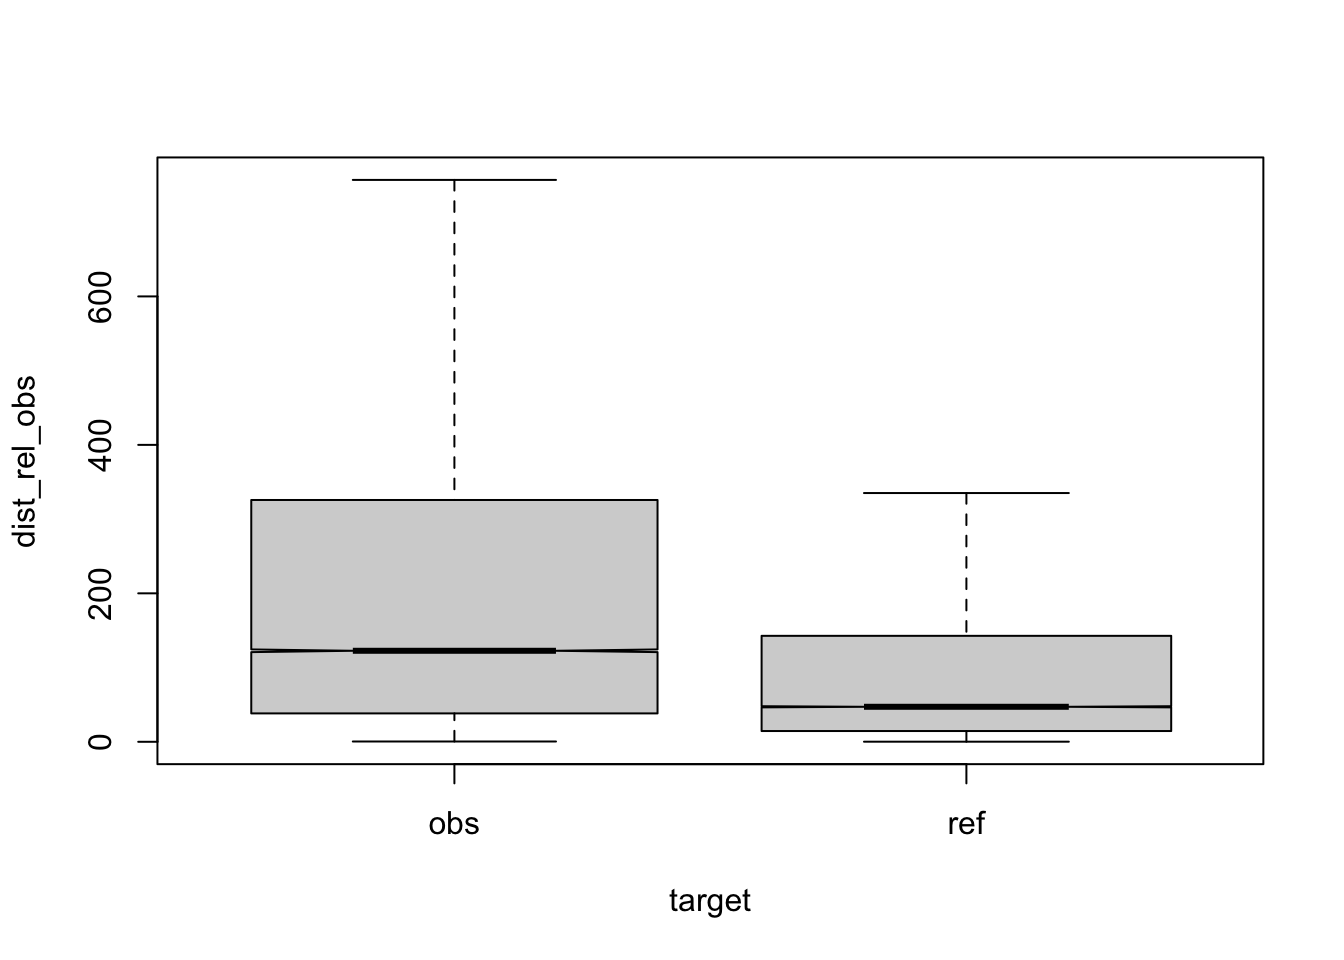
\includegraphics{spund-pub_files/figure-latex/boxplot11-1} \caption{compare distances by corpus, normalised to obs, distance ceiling =  outliers removed}\label{fig:boxplot11}
\end{figure}

\begin{figure}[H]
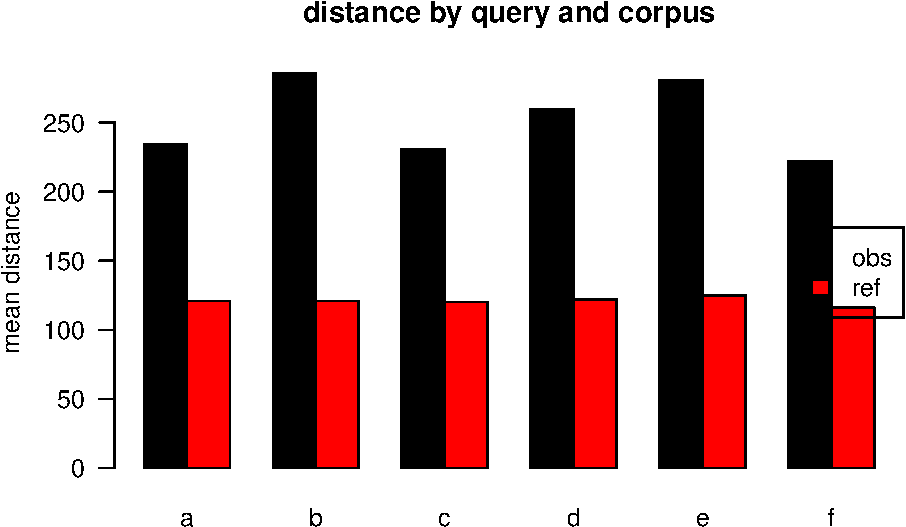
\includegraphics{spund-pub_files/figure-latex/barplot-mean1-1} \caption{mean distances over query/corpus, normalised to obs, distance ceiling =  outliers removed}\label{fig:barplot-mean1}
\end{figure}

\begin{longtable}[]{@{}llrrr@{}}
\caption{\label{tab:dfe-table1}mean/median table for model: 1}\tabularnewline
\toprule\noalign{}
target & q & n & mean & median \\
\midrule\noalign{}
\endfirsthead
\toprule\noalign{}
target & q & n & mean & median \\
\midrule\noalign{}
\endhead
\bottomrule\noalign{}
\endlastfoot
obs & a & 42836 & 234 & 117 \\
ref & a & 58615 & 121 & 47 \\
obs & b & 2116 & 286 & 165 \\
ref & b & 1130 & 121 & 44 \\
obs & c & 5770 & 231 & 114 \\
ref & c & 1274 & 120 & 48 \\
obs & d & 5654 & 260 & 144 \\
ref & d & 1525 & 122 & 49 \\
obs & e & 3911 & 281 & 147 \\
ref & e & 671 & 125 & 45 \\
obs & f & 2311 & 222 & 133 \\
ref & f & 413 & 116 & 47 \\
\end{longtable}

\begin{figure}[H]
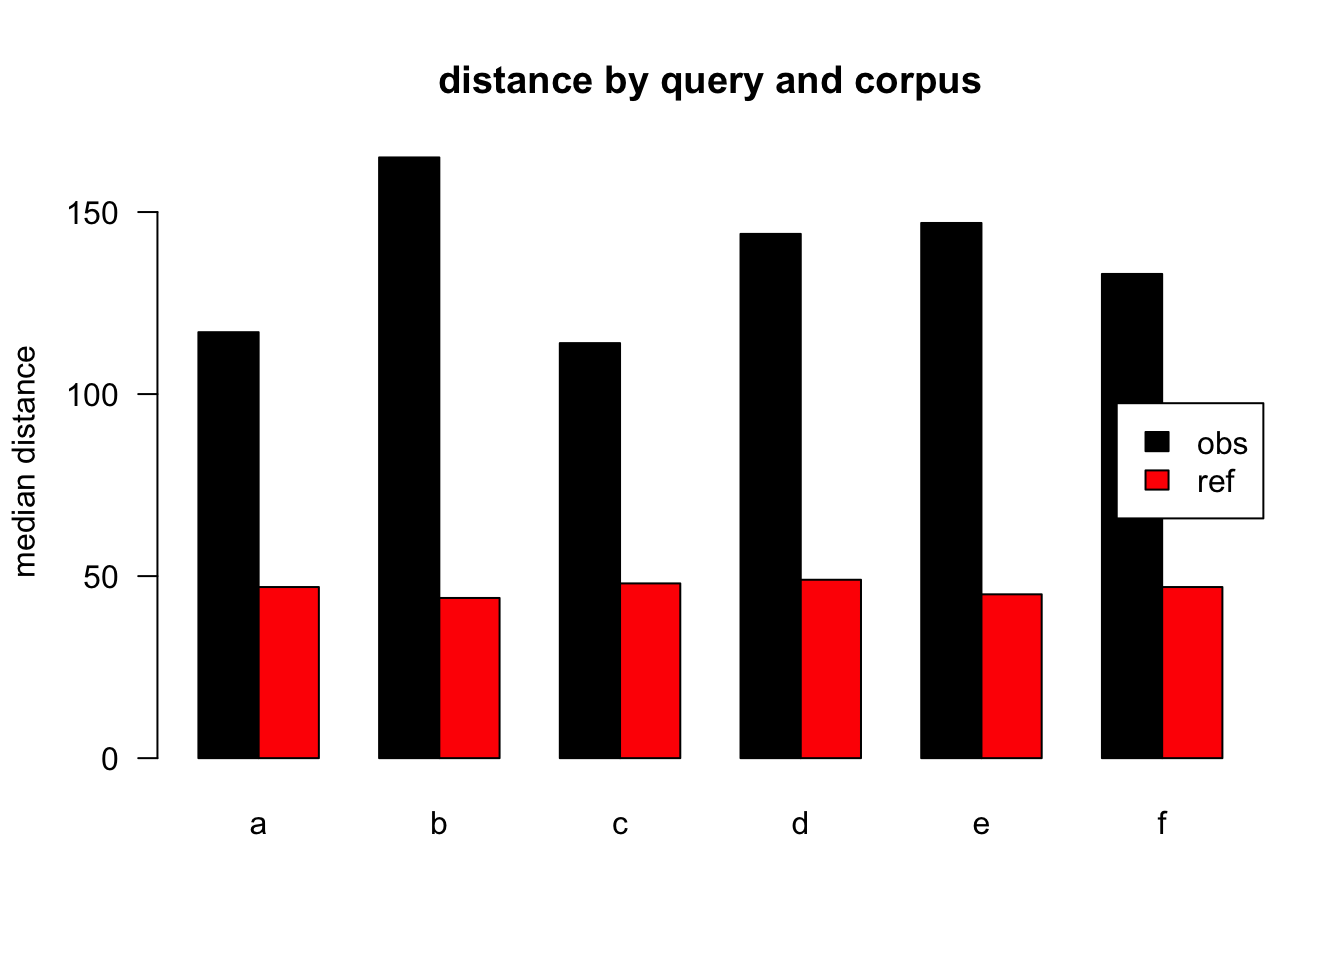
\includegraphics{spund-pub_files/figure-latex/barplot-median1-1} \caption{median distances over query/corpus, normalised to obs, distance ceiling =  outliers removed}\label{fig:barplot-median1}
\end{figure}

\begin{figure}[H]
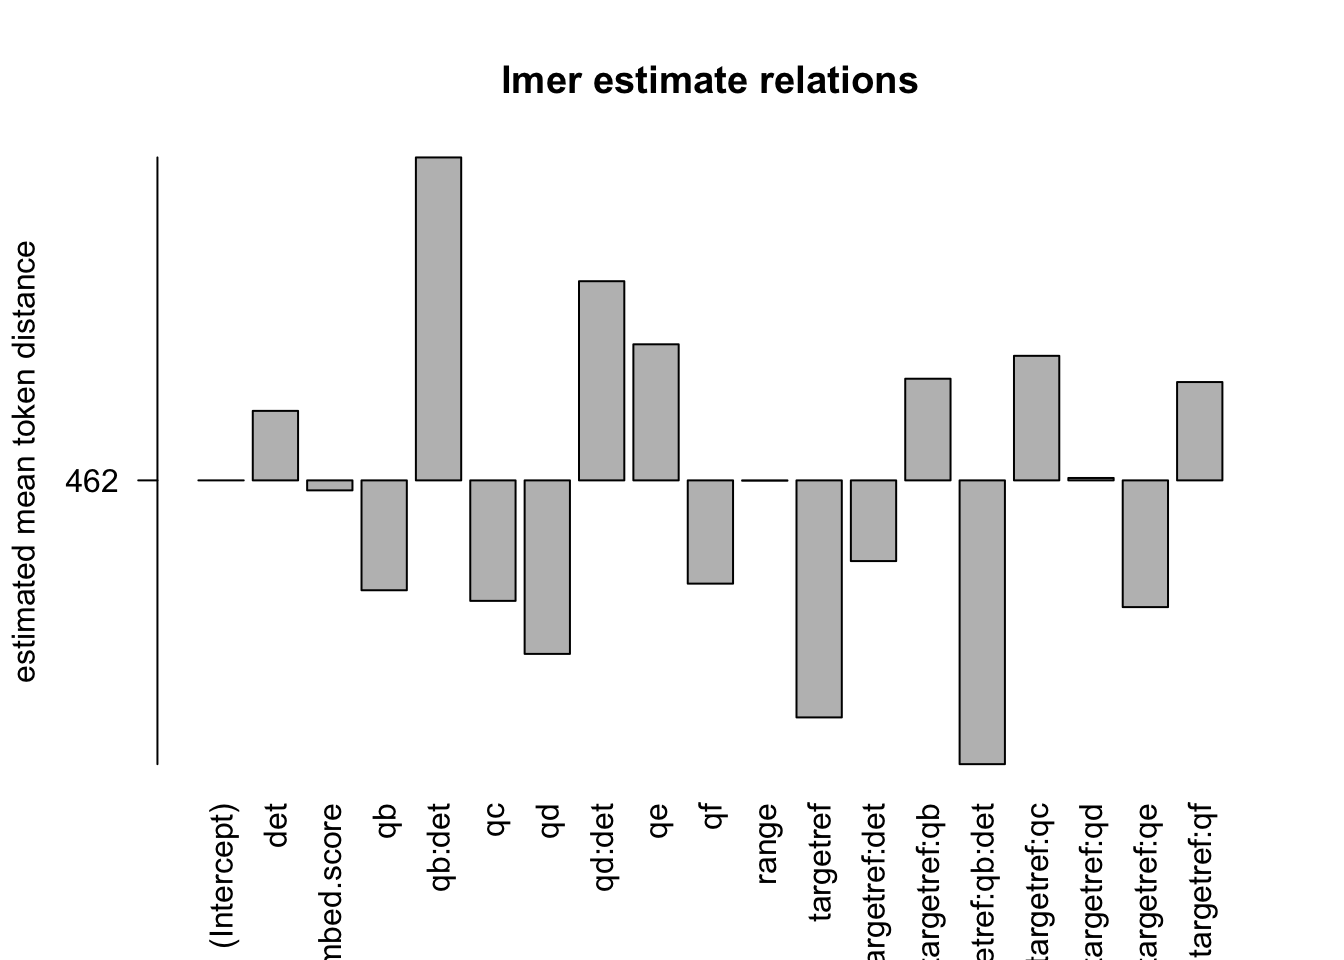
\includegraphics{spund-pub_files/figure-latex/lmeplot1-1} \caption{distances relation, normalised to obs, distance ceiling =  outliers removed}\label{fig:lmeplot1}
\end{figure}

\begin{figure}[H]
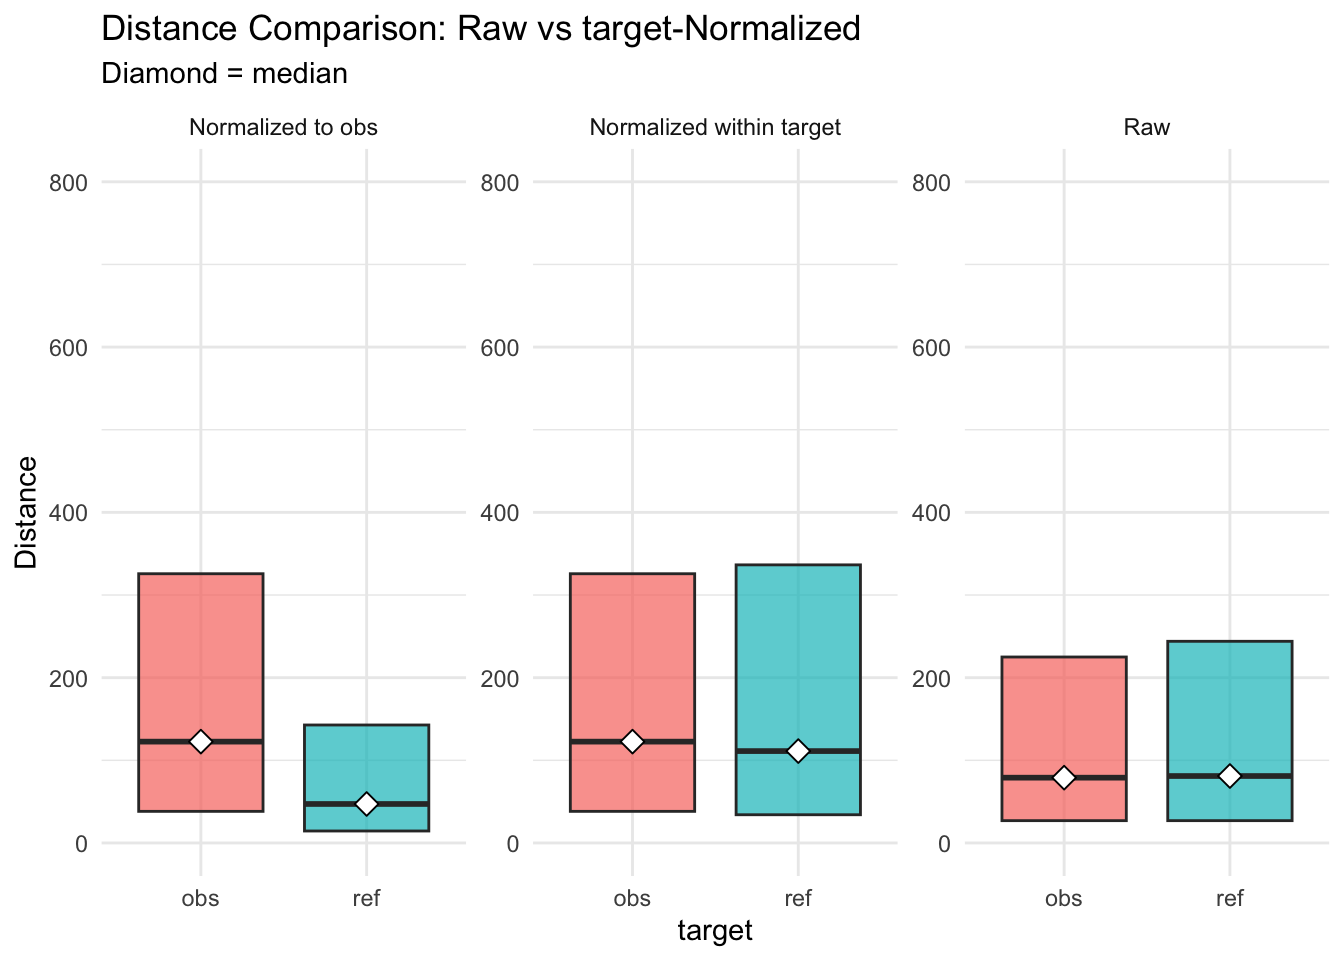
\includegraphics{spund-pub_files/figure-latex/gplot1-1} \caption{distances normalised vs. raw}\label{fig:gplot1}
\end{figure}

\section{evaluation model: 2}\label{evaluation-model-2}

\subsection{meta}\label{meta-1}

eval output data: 13, not normalised, distance ceiling =outliers not removed

\subsection{parameter setting}\label{parameter-setting-1}

\begin{verbatim}
##             value
## norm_target      
## det.t        TRUE
## limit       FALSE
## author       TRUE
## url          TRUE
## embed1       TRUE
## embed2          f
## range1       TRUE
## range2          f
## rel         FALSE
## lme         FALSE
## lemma       FALSE
\end{verbatim}

\subsection{anova analysis}\label{anova-analysis-1}

\subsubsection{anova plain}\label{anova-plain-1}

formula: {[}\texttt{dist\ \textasciitilde{}\ target*q*det}{]}

\begin{verbatim}
##                  Df     Sum Sq    Mean Sq  F value  Pr(>F)    
## target            1 1.1152e+11 1.1152e+11 268.8154 < 2e-16 ***
## q                 5 9.8792e+08 1.9758e+08   0.4763 0.79425    
## det               1 4.1537e+08 4.1537e+08   1.0012 0.31702    
## target:q          5 2.3050e+09 4.6101e+08   1.1112 0.35184    
## target:det        1 2.7199e+09 2.7199e+09   6.5561 0.01045 *  
## q:det             2 2.4028e+08 1.2014e+08   0.2896 0.74857    
## target:q:det      1 7.0024e+06 7.0024e+06   0.0169 0.89663    
## Residuals    142304 5.9037e+13 4.1487e+08                     
## ---
## Signif. codes:  0 '***' 0.001 '**' 0.01 '*' 0.05 '.' 0.1 ' ' 1
\end{verbatim}

\subsubsection{anova of linear regression model}\label{anova-of-linear-regression-model-1}

{[}\texttt{anova(summary(lmer))}{]}

\begin{verbatim}
## Type III Analysis of Variance Table with Satterthwaite's method
##                  Sum Sq    Mean Sq NumDF  DenDF  F value  Pr(>F)    
## target       1.2717e+09 1.2717e+09     1   3751   5.5781 0.01824 *  
## q            6.3534e+08 1.2707e+08     5 137654   0.5574 0.73281    
## det          7.3359e+05 7.3359e+05     1 133172   0.0032 0.95476    
## range        2.8637e+07 2.8637e+07     1   2113   0.1256 0.72306    
## embed.score  2.7199e+10 2.7199e+10     1 141732 119.3005 < 2e-16 ***
## target:q     3.0753e+09 6.1507e+08     5 138840   2.6979 0.01920 *  
## target:det   8.1028e+08 8.1028e+08     1 138434   3.5541 0.05940 .  
## q:det        4.8717e+08 2.4358e+08     2 135770   1.0684 0.34355    
## target:q:det 2.4585e+06 2.4585e+06     1 138496   0.0108 0.91729    
## ---
## Signif. codes:  0 '***' 0.001 '**' 0.01 '*' 0.05 '.' 0.1 ' ' 1
\end{verbatim}

\subsubsection{linear regression coefficients}\label{linear-regression-coefficients-1}

formula: {[}\texttt{dist\ \textasciitilde{}\ target*q*det+(1\textbar{}aut\_id)+range+(embed.score)+(1\textbar{}url\_id)}{]}

\begin{verbatim}
## Linear mixed model fit by REML. t-tests use Satterthwaite's method [
## lmerModLmerTest]
## Formula: eval(expr(lmeform))
##    Data: dfa
## 
## REML criterion at convergence: 3153644
## 
## Scaled residuals: 
##     Min      1Q  Median      3Q     Max 
## -23.760  -0.034  -0.006   0.025  55.672 
## 
## Random effects:
##  Groups   Name        Variance  Std.Dev.
##  aut_id   (Intercept)  28985985  5384   
##  url_id   (Intercept)  98381104  9919   
##  Residual             227983636 15099   
## Number of obs: 142321, groups:  aut_id, 8395; url_id, 2145
## 
## Fixed effects:
##                    Estimate Std. Error         df t value Pr(>|t|)    
## (Intercept)       2.873e+03  4.211e+02  8.594e+03   6.823 9.53e-12 ***
## targetref         1.341e+03  6.536e+02  2.412e+03   2.051   0.0404 *  
## qb                6.895e+01  1.008e+03  1.363e+05   0.068   0.9454    
## qc               -6.307e+02  3.622e+02  1.372e+05  -1.741   0.0816 .  
## qd               -1.993e+03  1.522e+04  1.332e+05  -0.131   0.8958    
## qe               -1.006e+02  2.520e+02  1.385e+05  -0.399   0.6899    
## qf               -1.355e+02  3.218e+02  1.384e+05  -0.421   0.6737    
## det               7.031e+02  3.145e+02  1.375e+05   2.236   0.0254 *  
## range             6.798e-02  1.918e-01  2.113e+03   0.354   0.7231    
## embed.score      -5.793e+03  5.304e+02  1.417e+05 -10.922  < 2e-16 ***
## targetref:qb      6.675e+02  1.124e+03  1.371e+05   0.594   0.5527    
## targetref:qc      3.752e+01  8.128e+02  1.395e+05   0.046   0.9632    
## targetref:qd      2.022e+03  7.989e+02  1.395e+05   2.531   0.0114 *  
## targetref:qe      2.269e+02  6.042e+02  1.395e+05   0.376   0.7073    
## targetref:qf      3.210e+02  7.643e+02  1.393e+05   0.420   0.6745    
## targetref:det    -1.416e+03  6.890e+02  1.397e+05  -2.055   0.0398 *  
## qb:det           -1.077e+03  1.107e+03  1.364e+05  -0.973   0.3304    
## qd:det            1.039e+03  1.521e+04  1.332e+05   0.068   0.9456    
## targetref:qb:det -1.651e+02  1.590e+03  1.385e+05  -0.104   0.9173    
## ---
## Signif. codes:  0 '***' 0.001 '**' 0.01 '*' 0.05 '.' 0.1 ' ' 1
## fit warnings:
## fixed-effect model matrix is rank deficient so dropping 7 columns / coefficients
## Some predictor variables are on very different scales: consider rescaling
\end{verbatim}

\subsection{plots}\label{plots-1}

\begin{figure}[H]
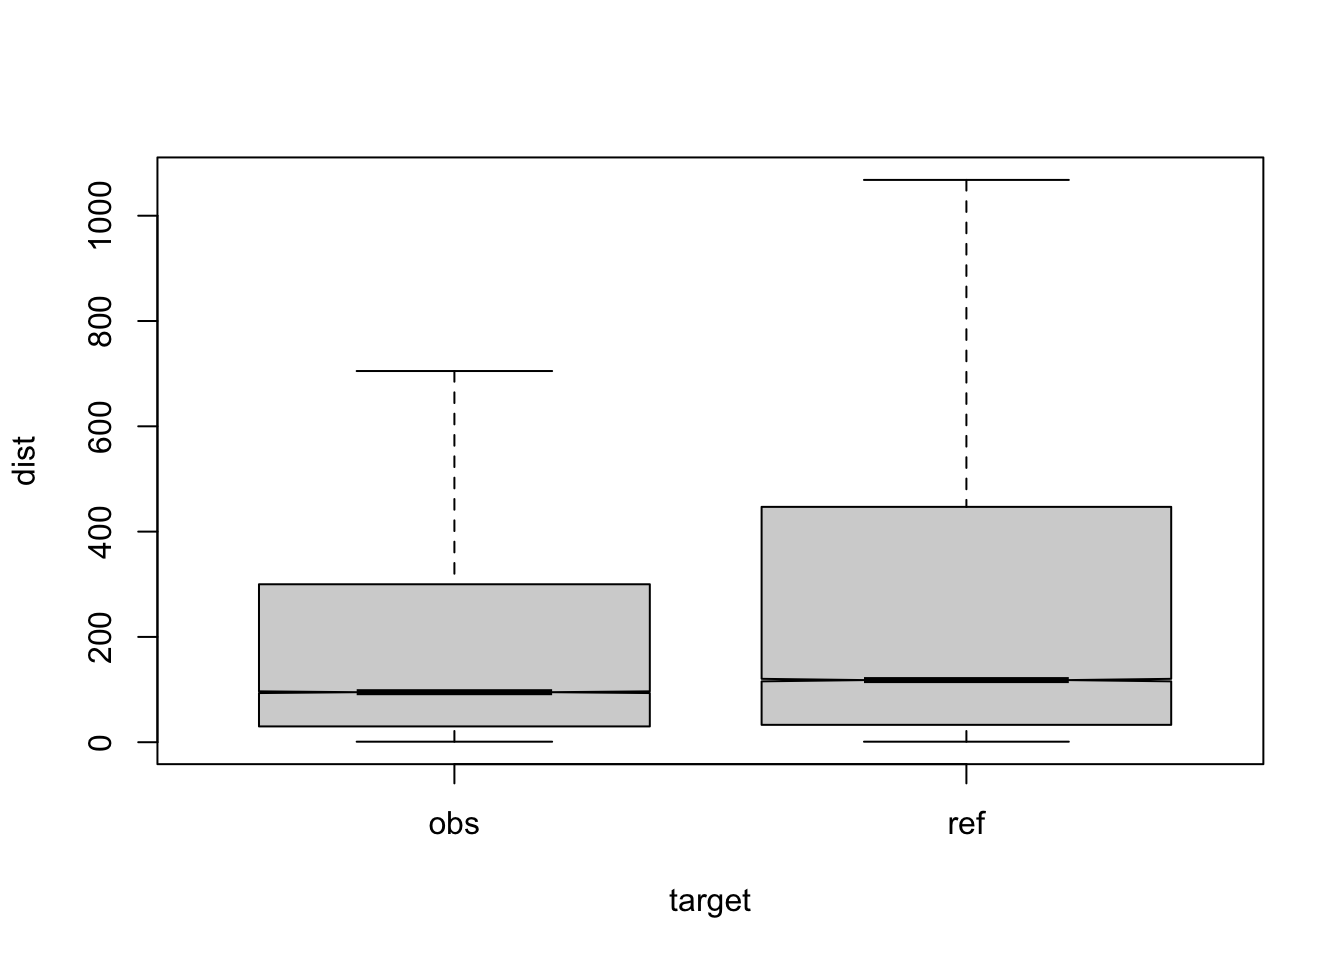
\includegraphics{spund-pub_files/figure-latex/boxplot12-1} \caption{compare distances by corpus, not normalised, distance ceiling =outliers not removed}\label{fig:boxplot12}
\end{figure}

\begin{figure}[H]
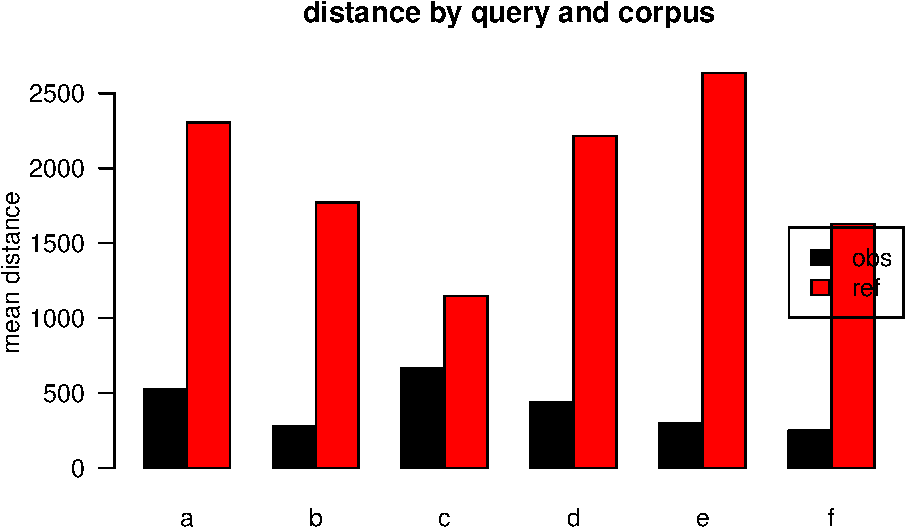
\includegraphics{spund-pub_files/figure-latex/barplot-mean2-1} \caption{mean distances over query/corpus, not normalised, distance ceiling =outliers not removed}\label{fig:barplot-mean2}
\end{figure}

\begin{longtable}[]{@{}llrrr@{}}
\caption{\label{tab:dfe-table2}mean/median table for model: 2}\tabularnewline
\toprule\noalign{}
target & q & n & mean & median \\
\midrule\noalign{}
\endfirsthead
\toprule\noalign{}
target & q & n & mean & median \\
\midrule\noalign{}
\endhead
\bottomrule\noalign{}
\endlastfoot
obs & a & 46318 & 525 & 92 \\
ref & a & 68618 & 2305 & 118 \\
obs & b & 2287 & 275 & 109 \\
ref & b & 1315 & 1771 & 111 \\
obs & c & 6253 & 666 & 89 \\
ref & c & 1504 & 1147 & 119 \\
obs & d & 6171 & 441 & 105 \\
ref & d & 1765 & 2214 & 124 \\
obs & e & 4278 & 298 & 109 \\
ref & e & 795 & 2636 & 116 \\
obs & f & 2520 & 249 & 77 \\
ref & f & 497 & 1627 & 124 \\
\end{longtable}

\begin{figure}[H]
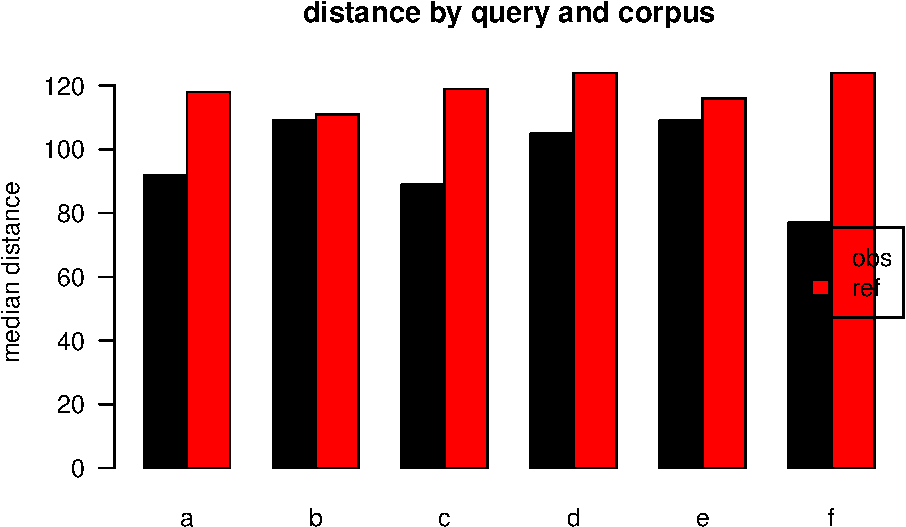
\includegraphics{spund-pub_files/figure-latex/barplot-median2-1} \caption{median distances over query/corpus, not normalised, distance ceiling =outliers not removed}\label{fig:barplot-median2}
\end{figure}

\begin{figure}[H]
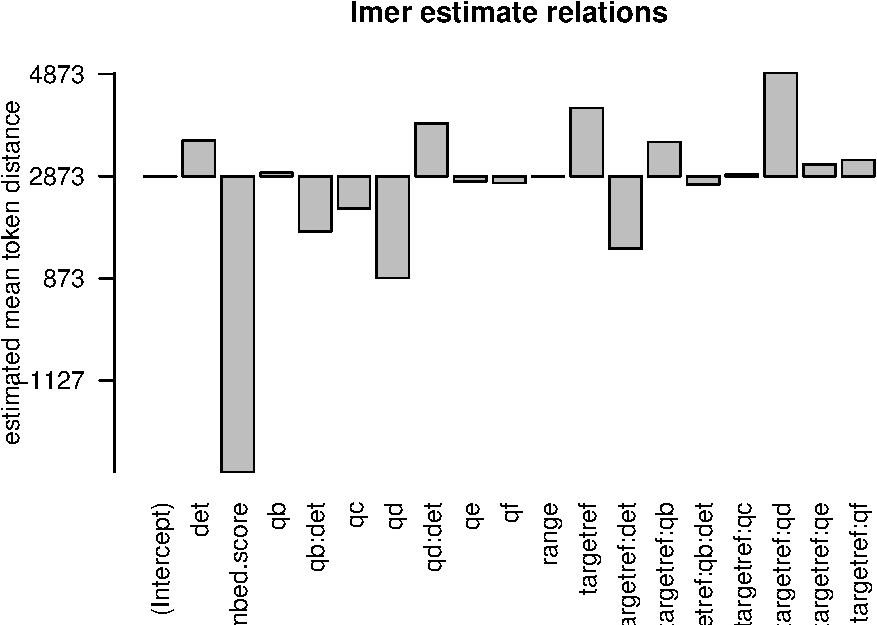
\includegraphics{spund-pub_files/figure-latex/lmeplot2-1} \caption{distances relation, not normalised, distance ceiling =outliers not removed}\label{fig:lmeplot2}
\end{figure}

\begin{figure}[H]
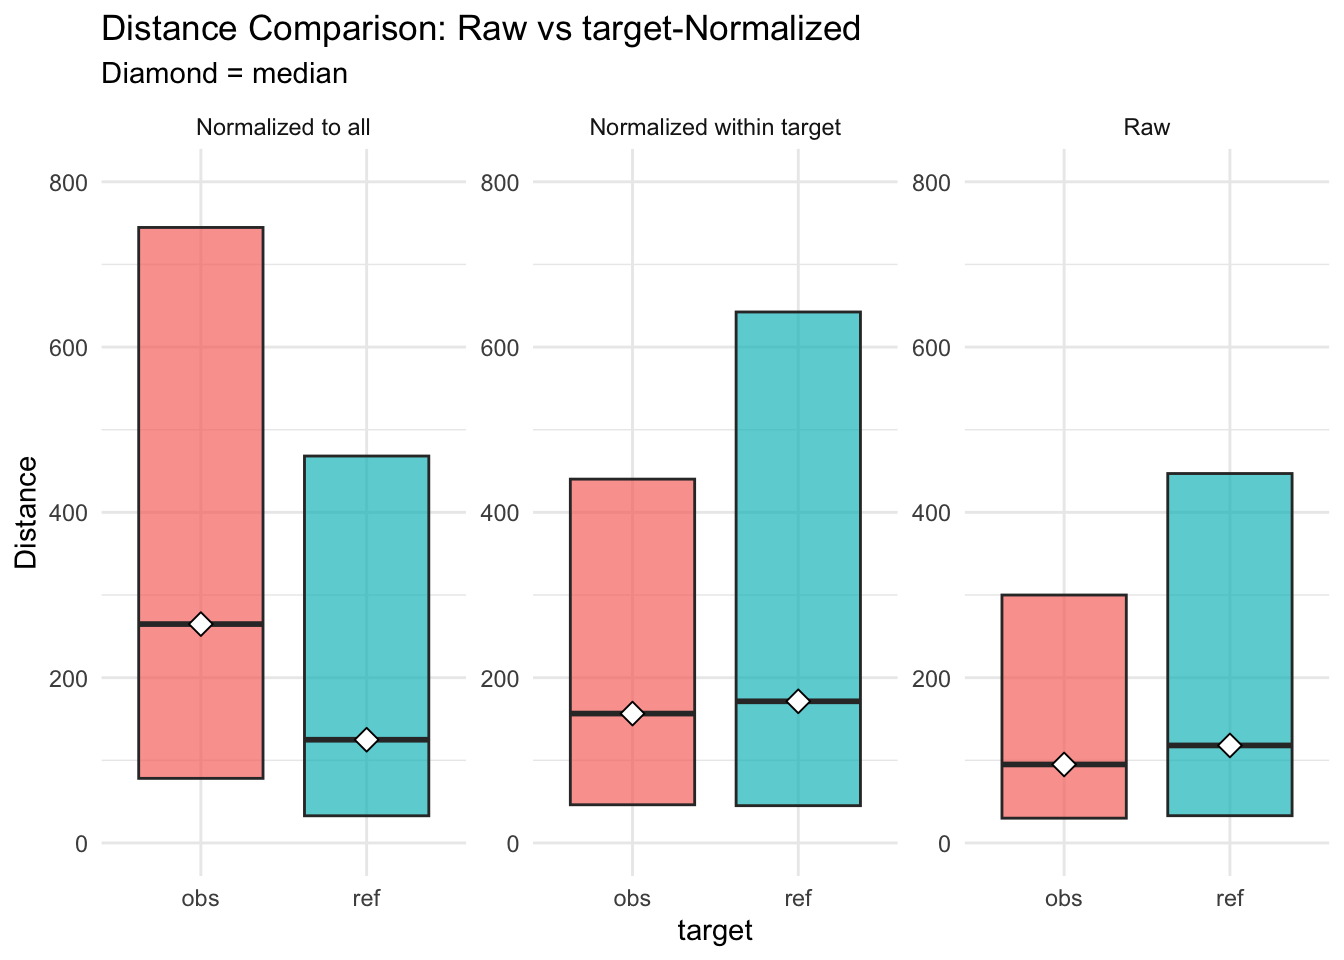
\includegraphics{spund-pub_files/figure-latex/gplot2-1} \caption{distances normalised vs. raw}\label{fig:gplot2}
\end{figure}

\section{evaluation model: 3}\label{evaluation-model-3}

\subsection{meta}\label{meta-2}

eval output data: 13, normalised to all, distance ceiling = outliers removed

\subsection{parameter setting}\label{parameter-setting-2}

\begin{verbatim}
##                value
## norm_target _rel_all
## det.t           TRUE
## limit           TRUE
## author          TRUE
## url             TRUE
## embed1          TRUE
## embed2             f
## range1          TRUE
## range2             f
## rel             TRUE
## lme            FALSE
## lemma          FALSE
\end{verbatim}

\subsection{anova analysis}\label{anova-analysis-2}

\subsubsection{anova plain}\label{anova-plain-2}

formula: {[}\texttt{dist\_rel\_all\ \textasciitilde{}\ target*q*det}{]}

\begin{verbatim}
##                  Df     Sum Sq    Mean Sq   F value    Pr(>F)    
## target            1 1.2830e+09 1283010757 7336.4625 < 2.2e-16 ***
## q                 5 3.4949e+07    6989793   39.9688 < 2.2e-16 ***
## det               1 4.6410e+06    4641007   26.5380 2.588e-07 ***
## target:q          5 7.7932e+06    1558646    8.9126 1.786e-08 ***
## target:det        1 7.1283e+05     712833    4.0761  0.043496 *  
## q:det             2 2.5680e+06    1283981    7.3420  0.000648 ***
## target:q:det      1 2.0345e+06    2034482   11.6335  0.000648 ***
## Residuals    126209 2.2072e+10     174881                        
## ---
## Signif. codes:  0 '***' 0.001 '**' 0.01 '*' 0.05 '.' 0.1 ' ' 1
\end{verbatim}

\subsubsection{anova of linear regression model}\label{anova-of-linear-regression-model-2}

{[}\texttt{anova(summary(lmer))}{]}

\begin{verbatim}
## Type III Analysis of Variance Table with Satterthwaite's method
##                 Sum Sq   Mean Sq NumDF  DenDF   F value    Pr(>F)    
## target         3245706   3245706     1   3519   23.4567 1.333e-06 ***
## q              2091953    418391     5 122421    3.0237 0.0098706 ** 
## det              34508     34508     1 118425    0.2494 0.6175055    
## range        142964301 142964301     1   1025 1033.2042 < 2.2e-16 ***
## embed.score   71204325  71204325     1 122690  514.5942 < 2.2e-16 ***
## target:q       2202162    440432     5 123486    3.1830 0.0070933 ** 
## target:det     1534830   1534830     1 123325   11.0922 0.0008672 ***
## q:det          1019818    509909     2 120804    3.6851 0.0250971 *  
## target:q:det    623611    623611     1 123315    4.5068 0.0337615 *  
## ---
## Signif. codes:  0 '***' 0.001 '**' 0.01 '*' 0.05 '.' 0.1 ' ' 1
\end{verbatim}

\subsubsection{linear regression coefficients}\label{linear-regression-coefficients-2}

formula: {[}\texttt{dist\_rel\_all\ \textasciitilde{}\ target*q*det+(1\textbar{}aut\_id)+range+(embed.score)+(1\textbar{}url\_id)}{]}

\begin{verbatim}
## Linear mixed model fit by REML. t-tests use Satterthwaite's method [
## lmerModLmerTest]
## Formula: eval(expr(lmeform))
##    Data: dfa
## 
## REML criterion at convergence: 1859224
## 
## Scaled residuals: 
##     Min      1Q  Median      3Q     Max 
## -2.8643 -0.5282 -0.1721  0.2469  6.9244 
## 
## Random effects:
##  Groups   Name        Variance Std.Dev.
##  aut_id   (Intercept)   8101    90.01  
##  url_id   (Intercept)  23223   152.39  
##  Residual             138370   371.98  
## Number of obs: 126226, groups:  aut_id, 8238; url_id, 2145
## 
## Fixed effects:
##                    Estimate Std. Error         df t value Pr(>|t|)    
## (Intercept)       7.789e+02  8.688e+00  8.969e+03  89.651  < 2e-16 ***
## targetref        -7.312e+01  1.061e+01  1.300e+03  -6.893 8.50e-12 ***
## qb               -3.390e+01  2.572e+01  1.218e+05  -1.318 0.187483    
## qc               -3.717e+01  9.261e+00  1.226e+05  -4.014 5.98e-05 ***
## qd               -5.353e+01  3.748e+02  1.184e+05  -0.143 0.886426    
## qe                4.198e+01  6.460e+00  1.247e+05   6.498 8.14e-11 ***
## qf               -3.185e+01  8.240e+00  1.244e+05  -3.866 0.000111 ***
## det               2.144e+01  8.041e+00  1.229e+05   2.667 0.007662 ** 
## range            -9.786e-02  3.044e-03  1.025e+03 -32.143  < 2e-16 ***
## embed.score      -3.080e+02  1.358e+01  1.227e+05 -22.685  < 2e-16 ***
## targetref:qb      3.136e+01  2.894e+01  1.225e+05   1.083 0.278599    
## targetref:qc      3.842e+01  2.154e+01  1.237e+05   1.784 0.074435 .  
## targetref:qd      7.432e-01  2.113e+01  1.238e+05   0.035 0.971935    
## targetref:qe     -3.910e+01  1.602e+01  1.239e+05  -2.441 0.014662 *  
## targetref:qf      3.033e+01  2.039e+01  1.238e+05   1.488 0.136766    
## targetref:det    -2.490e+01  1.826e+01  1.239e+05  -1.363 0.172784    
## qb:det            9.962e+01  2.826e+01  1.219e+05   3.526 0.000423 ***
## qd:det            6.144e+01  3.747e+02  1.184e+05   0.164 0.869736    
## targetref:qb:det -8.754e+01  4.124e+01  1.233e+05  -2.123 0.033761 *  
## ---
## Signif. codes:  0 '***' 0.001 '**' 0.01 '*' 0.05 '.' 0.1 ' ' 1
## fit warnings:
## fixed-effect model matrix is rank deficient so dropping 7 columns / coefficients
## Some predictor variables are on very different scales: consider rescaling
\end{verbatim}

\subsection{plots}\label{plots-2}

\begin{figure}[H]
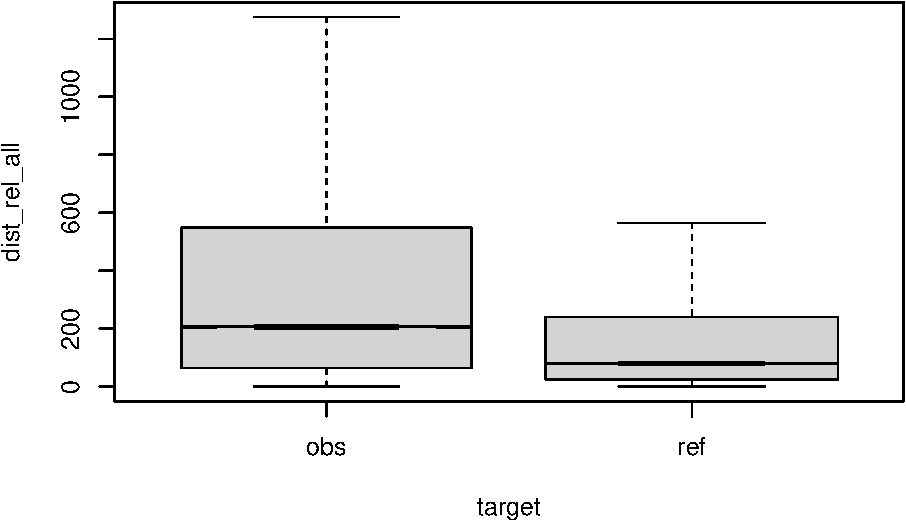
\includegraphics{spund-pub_files/figure-latex/boxplot13-1} \caption{compare distances by corpus, normalised to all, distance ceiling =  outliers removed}\label{fig:boxplot13}
\end{figure}

\begin{figure}[H]
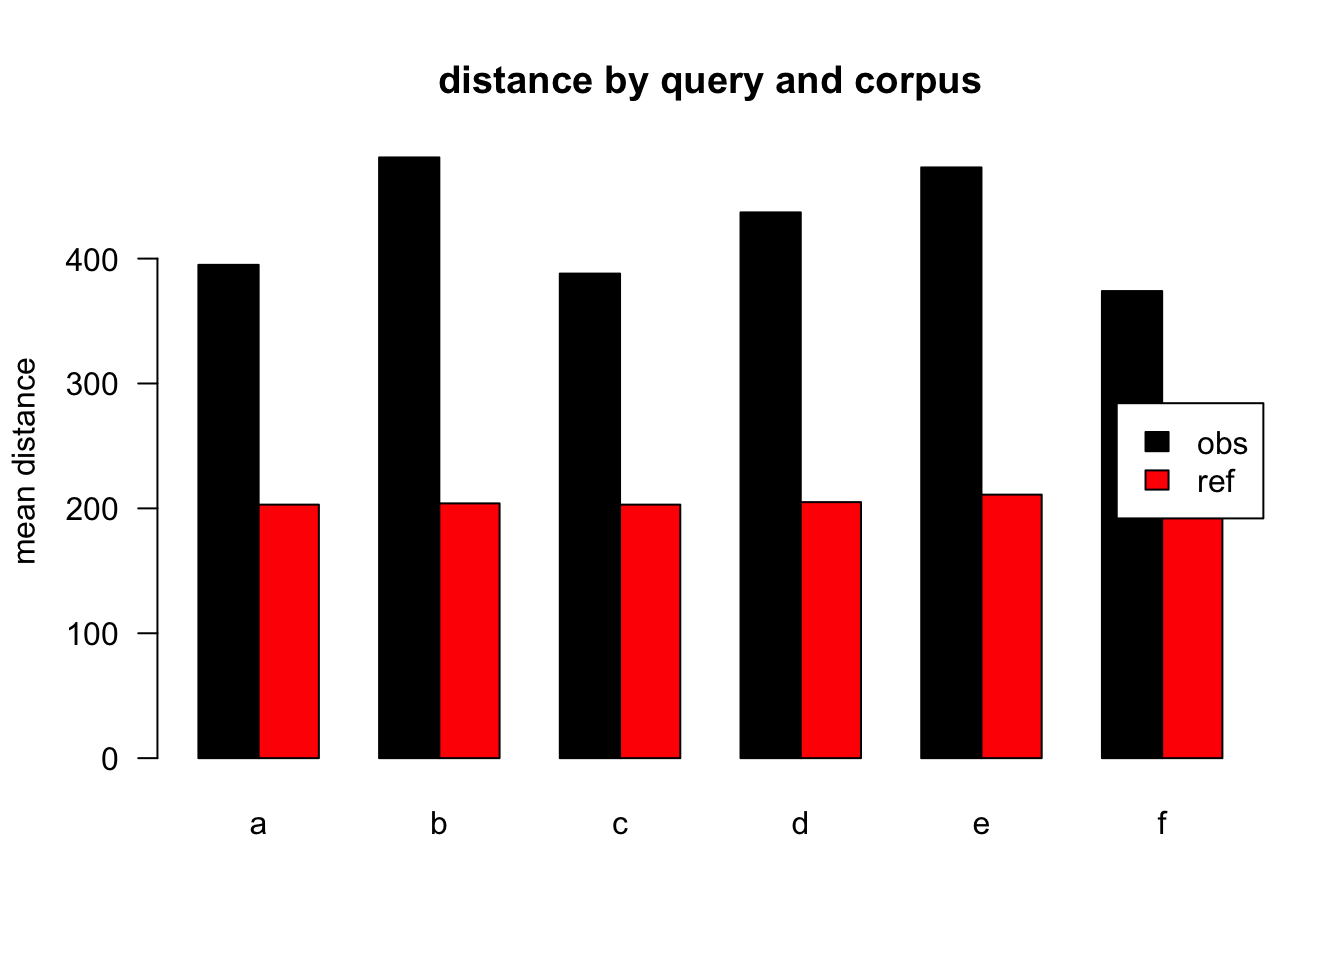
\includegraphics{spund-pub_files/figure-latex/barplot-mean3-1} \caption{mean distances over query/corpus, normalised to all, distance ceiling =  outliers removed}\label{fig:barplot-mean3}
\end{figure}

\begin{longtable}[]{@{}llrrr@{}}
\caption{\label{tab:dfe-table3}mean/median table for model: 3}\tabularnewline
\toprule\noalign{}
target & q & n & mean & median \\
\midrule\noalign{}
\endfirsthead
\toprule\noalign{}
target & q & n & mean & median \\
\midrule\noalign{}
\endhead
\bottomrule\noalign{}
\endlastfoot
obs & a & 42836 & 395 & 196 \\
ref & a & 58615 & 203 & 79 \\
obs & b & 2116 & 481 & 279 \\
ref & b & 1130 & 204 & 75 \\
obs & c & 5770 & 388 & 191 \\
ref & c & 1274 & 203 & 80 \\
obs & d & 5654 & 437 & 243 \\
ref & d & 1525 & 205 & 83 \\
obs & e & 3911 & 473 & 248 \\
ref & e & 671 & 211 & 75 \\
obs & f & 2311 & 374 & 224 \\
ref & f & 413 & 195 & 79 \\
\end{longtable}

\begin{figure}[H]
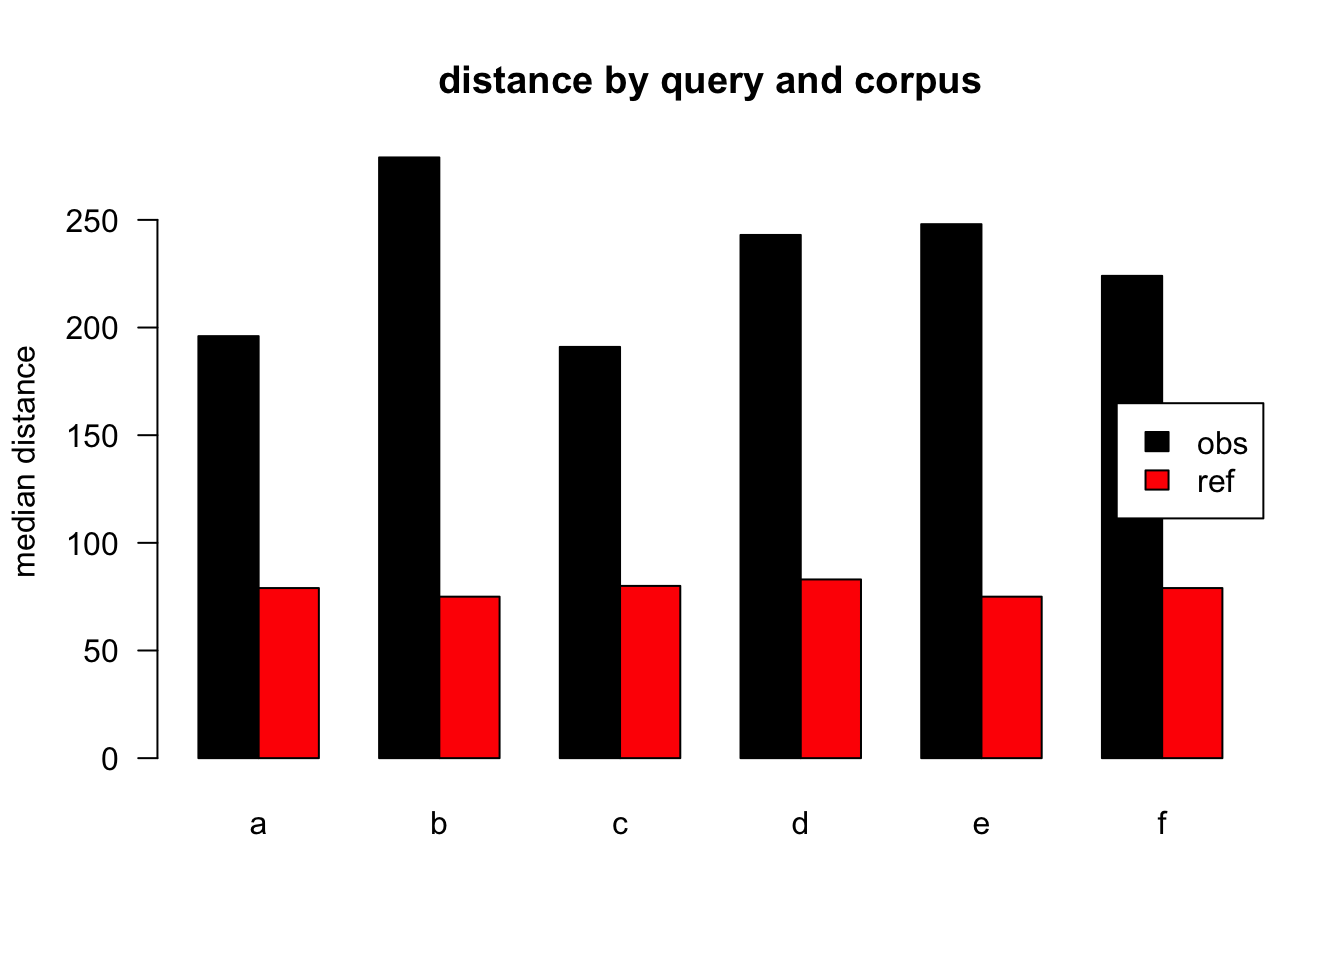
\includegraphics{spund-pub_files/figure-latex/barplot-median3-1} \caption{median distances over query/corpus, normalised to all, distance ceiling =  outliers removed}\label{fig:barplot-median3}
\end{figure}

\begin{figure}[H]
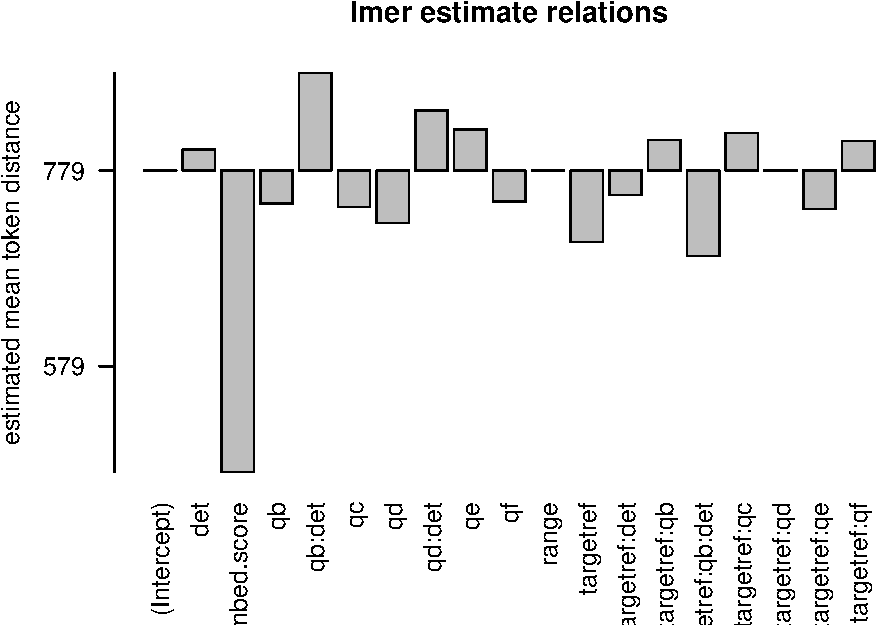
\includegraphics{spund-pub_files/figure-latex/lmeplot3-1} \caption{distances relation, normalised to all, distance ceiling =  outliers removed}\label{fig:lmeplot3}
\end{figure}

\begin{figure}[H]
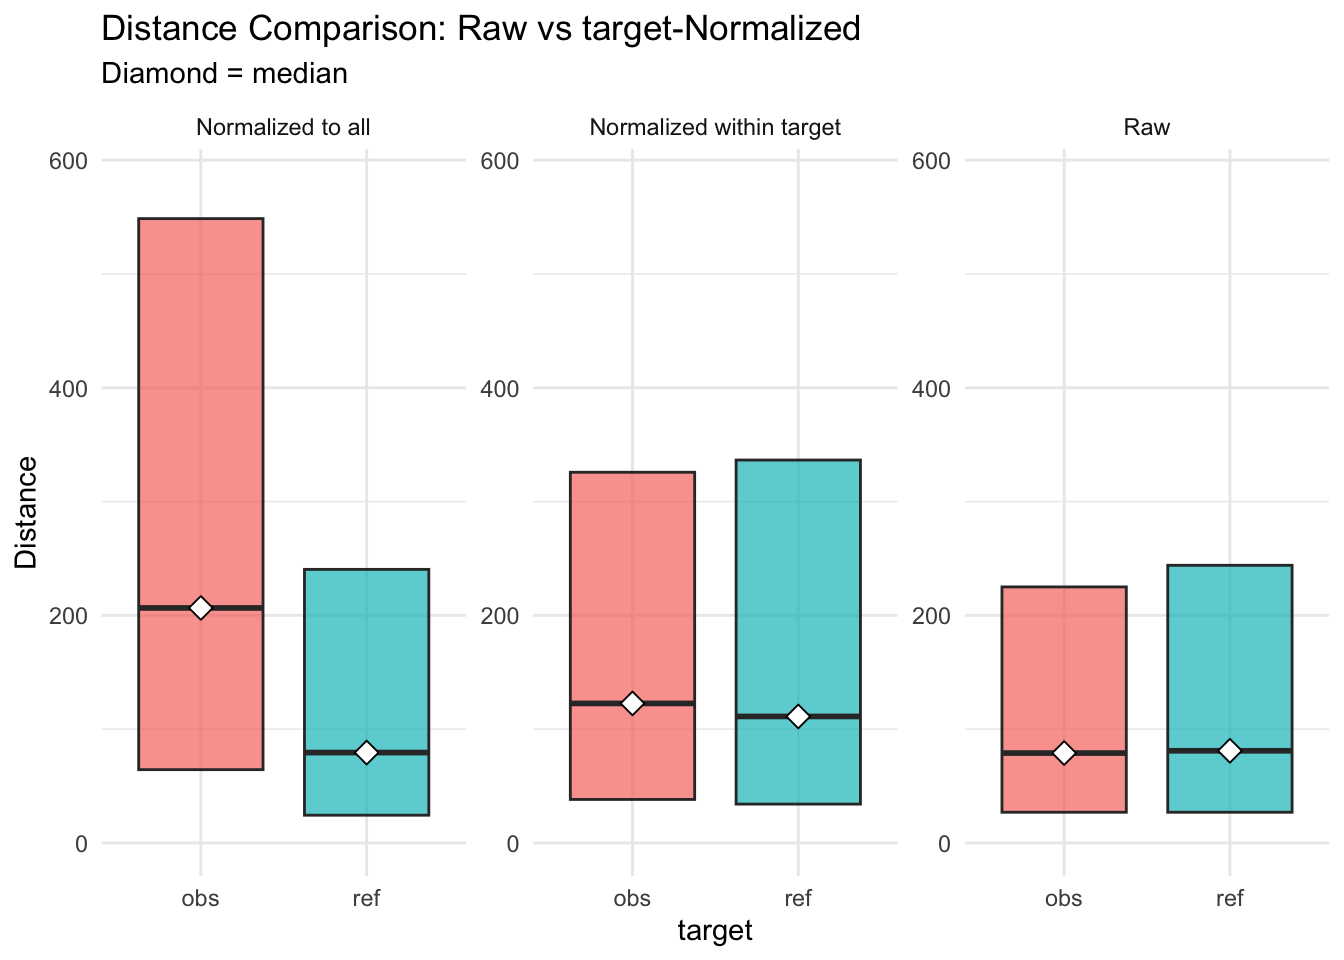
\includegraphics{spund-pub_files/figure-latex/gplot3-1} \caption{distances normalised vs. raw}\label{fig:gplot3}
\end{figure}

\section{evaluation model: 4}\label{evaluation-model-4}

\subsection{meta}\label{meta-3}

eval output data: 13, normalised to ref, distance ceiling = outliers removed

\subsection{parameter setting}\label{parameter-setting-3}

\begin{verbatim}
##                value
## norm_target _rel_ref
## det.t           TRUE
## limit           TRUE
## author          TRUE
## url             TRUE
## embed1          TRUE
## embed2             f
## range1          TRUE
## range2             f
## rel             TRUE
## lme            FALSE
## lemma          FALSE
\end{verbatim}

\subsection{anova analysis}\label{anova-analysis-3}

\subsubsection{anova plain}\label{anova-plain-3}

formula: {[}\texttt{dist\_rel\_ref\ \textasciitilde{}\ target*q*det}{]}

\begin{verbatim}
##                  Df     Sum Sq    Mean Sq   F value    Pr(>F)    
## target            1 2.5135e+09 2513546743 7336.4625 < 2.2e-16 ***
## q                 5 6.8469e+07   13693706   39.9688 < 2.2e-16 ***
## det               1 9.0922e+06    9092198   26.5380 2.588e-07 ***
## target:q          5 1.5268e+07    3053543    8.9126 1.786e-08 ***
## target:det        1 1.3965e+06    1396511    4.0761  0.043496 *  
## q:det             2 5.0309e+06    2515448    7.3420  0.000648 ***
## target:q:det      1 3.9858e+06    3985754   11.6335  0.000648 ***
## Residuals    126209 4.3240e+10     342610                        
## ---
## Signif. codes:  0 '***' 0.001 '**' 0.01 '*' 0.05 '.' 0.1 ' ' 1
\end{verbatim}

\subsubsection{anova of linear regression model}\label{anova-of-linear-regression-model-3}

{[}\texttt{anova(summary(lmer))}{]}

\begin{verbatim}
## Type III Analysis of Variance Table with Satterthwaite's method
##                 Sum Sq   Mean Sq NumDF  DenDF   F value    Pr(>F)    
## target         6358663   6358663     1   3519   23.4567 1.333e-06 ***
## q              4098347    819669     5 122421    3.0237 0.0098706 ** 
## det              67605     67605     1 118425    0.2494 0.6175055    
## range        280081403 280081403     1   1025 1033.2042 < 2.2e-16 ***
## embed.score  139496414 139496414     1 122690  514.5942 < 2.2e-16 ***
## target:q       4314256    862851     5 123486    3.1830 0.0070933 ** 
## target:det     3006886   3006886     1 123325   11.0922 0.0008672 ***
## q:det          1997926    998963     2 120804    3.6851 0.0250971 *  
## target:q:det   1221717   1221717     1 123315    4.5068 0.0337615 *  
## ---
## Signif. codes:  0 '***' 0.001 '**' 0.01 '*' 0.05 '.' 0.1 ' ' 1
\end{verbatim}

\subsubsection{linear regression coefficients}\label{linear-regression-coefficients-3}

formula: {[}\texttt{dist\_rel\_ref\ \textasciitilde{}\ target*q*det+(1\textbar{}aut\_id)+range+(embed.score)+(1\textbar{}url\_id)}{]}

\begin{verbatim}
## Linear mixed model fit by REML. t-tests use Satterthwaite's method [
## lmerModLmerTest]
## Formula: eval(expr(lmeform))
##    Data: dfa
## 
## REML criterion at convergence: 1944096
## 
## Scaled residuals: 
##     Min      1Q  Median      3Q     Max 
## -2.8643 -0.5282 -0.1721  0.2469  6.9244 
## 
## Random effects:
##  Groups   Name        Variance Std.Dev.
##  aut_id   (Intercept)  15871   126.0   
##  url_id   (Intercept)  45496   213.3   
##  Residual             271080   520.7   
## Number of obs: 126226, groups:  aut_id, 8238; url_id, 2145
## 
## Fixed effects:
##                    Estimate Std. Error         df t value Pr(>|t|)    
## (Intercept)       1.090e+03  1.216e+01  8.969e+03  89.651  < 2e-16 ***
## targetref        -1.024e+02  1.485e+01  1.300e+03  -6.893 8.50e-12 ***
## qb               -4.744e+01  3.600e+01  1.218e+05  -1.318 0.187483    
## qc               -5.203e+01  1.296e+01  1.226e+05  -4.014 5.98e-05 ***
## qd               -7.492e+01  5.246e+02  1.184e+05  -0.143 0.886426    
## qe                5.876e+01  9.042e+00  1.247e+05   6.498 8.14e-11 ***
## qf               -4.458e+01  1.153e+01  1.244e+05  -3.866 0.000111 ***
## det               3.001e+01  1.125e+01  1.229e+05   2.667 0.007662 ** 
## range            -1.370e-01  4.261e-03  1.025e+03 -32.143  < 2e-16 ***
## embed.score      -4.311e+02  1.900e+01  1.227e+05 -22.685  < 2e-16 ***
## targetref:qb      4.389e+01  4.051e+01  1.225e+05   1.083 0.278599    
## targetref:qc      5.378e+01  3.015e+01  1.237e+05   1.784 0.074435 .  
## targetref:qd      1.040e+00  2.957e+01  1.238e+05   0.035 0.971935    
## targetref:qe     -5.472e+01  2.242e+01  1.239e+05  -2.441 0.014662 *  
## targetref:qf      4.246e+01  2.853e+01  1.238e+05   1.488 0.136766    
## targetref:det    -3.485e+01  2.556e+01  1.239e+05  -1.363 0.172784    
## qb:det            1.394e+02  3.955e+01  1.219e+05   3.526 0.000423 ***
## qd:det            8.600e+01  5.244e+02  1.184e+05   0.164 0.869736    
## targetref:qb:det -1.225e+02  5.772e+01  1.233e+05  -2.123 0.033761 *  
## ---
## Signif. codes:  0 '***' 0.001 '**' 0.01 '*' 0.05 '.' 0.1 ' ' 1
## fit warnings:
## fixed-effect model matrix is rank deficient so dropping 7 columns / coefficients
## Some predictor variables are on very different scales: consider rescaling
\end{verbatim}

\subsection{plots}\label{plots-3}

\begin{figure}[H]
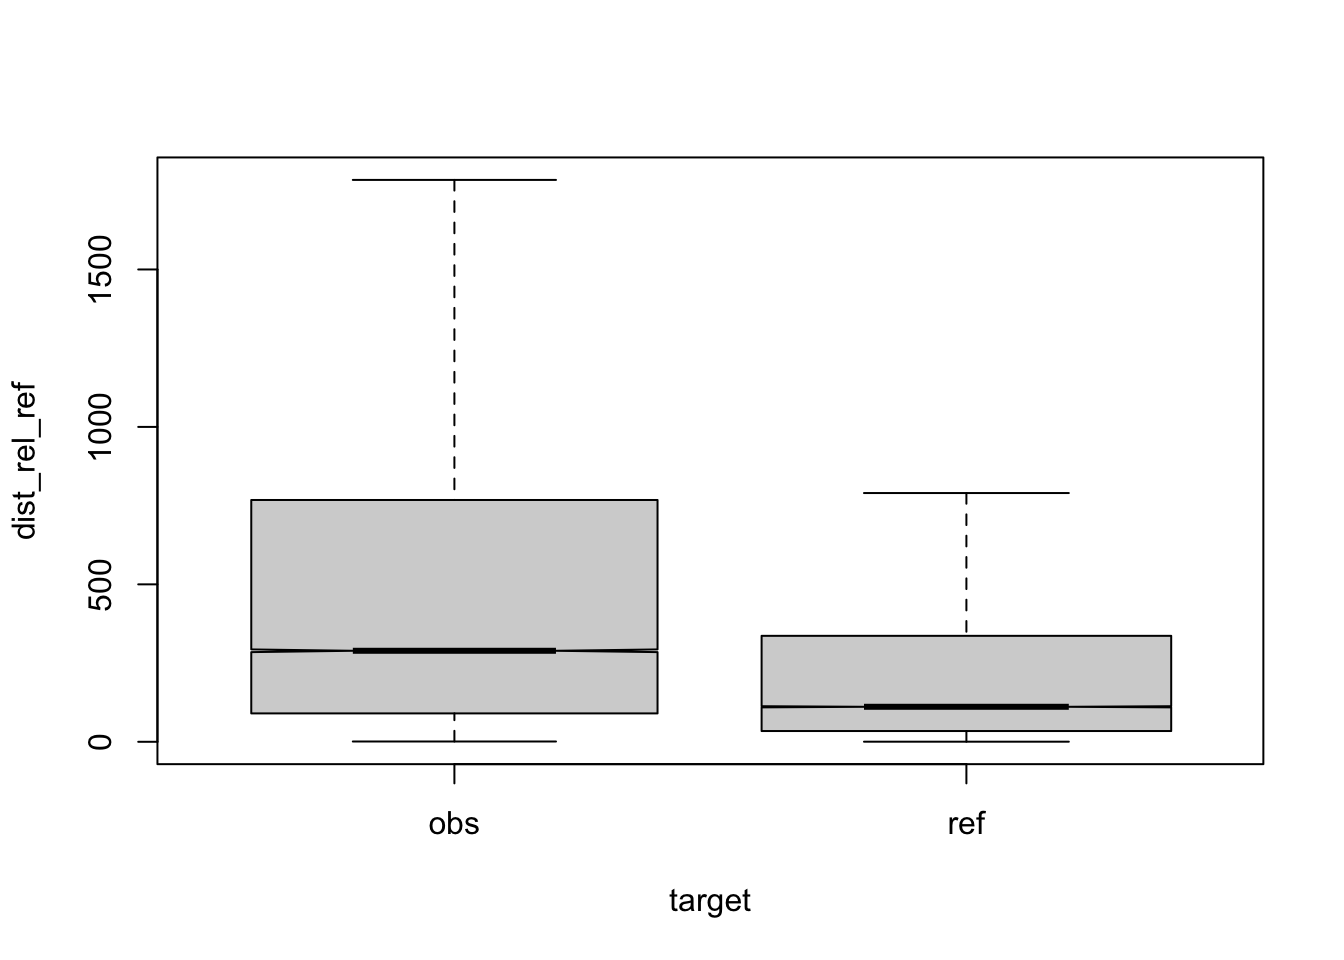
\includegraphics{spund-pub_files/figure-latex/boxplot14-1} \caption{compare distances by corpus, normalised to ref, distance ceiling =  outliers removed}\label{fig:boxplot14}
\end{figure}

\begin{figure}[H]
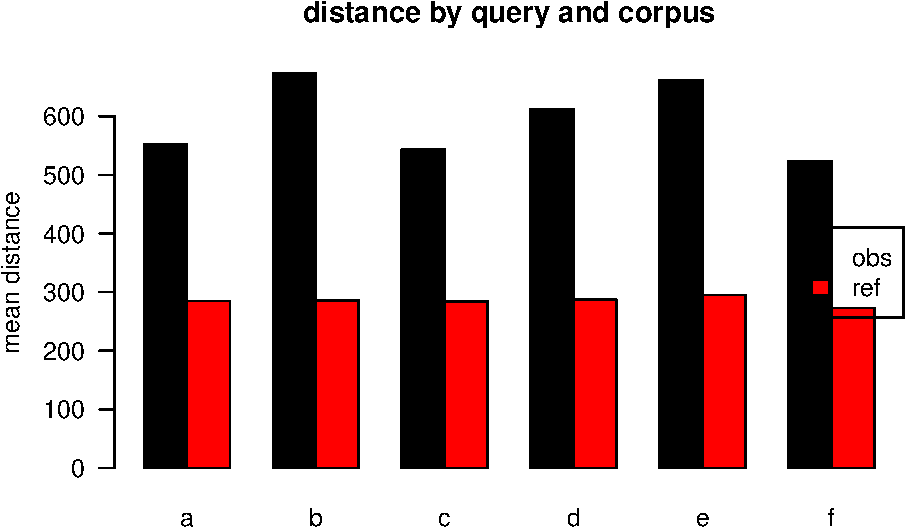
\includegraphics{spund-pub_files/figure-latex/barplot-mean4-1} \caption{mean distances over query/corpus, normalised to ref, distance ceiling =  outliers removed}\label{fig:barplot-mean4}
\end{figure}

\begin{longtable}[]{@{}llrrr@{}}
\caption{\label{tab:dfe-table4}mean/median table for model: 4}\tabularnewline
\toprule\noalign{}
target & q & n & mean & median \\
\midrule\noalign{}
\endfirsthead
\toprule\noalign{}
target & q & n & mean & median \\
\midrule\noalign{}
\endhead
\bottomrule\noalign{}
\endlastfoot
obs & a & 42836 & 553 & 275 \\
ref & a & 58615 & 285 & 111 \\
obs & b & 2116 & 674 & 390 \\
ref & b & 1130 & 286 & 104 \\
obs & c & 5770 & 543 & 268 \\
ref & c & 1274 & 284 & 112 \\
obs & d & 5654 & 612 & 340 \\
ref & d & 1525 & 287 & 116 \\
obs & e & 3911 & 662 & 347 \\
ref & e & 671 & 295 & 105 \\
obs & f & 2311 & 523 & 313 \\
ref & f & 413 & 273 & 111 \\
\end{longtable}

\begin{figure}[H]
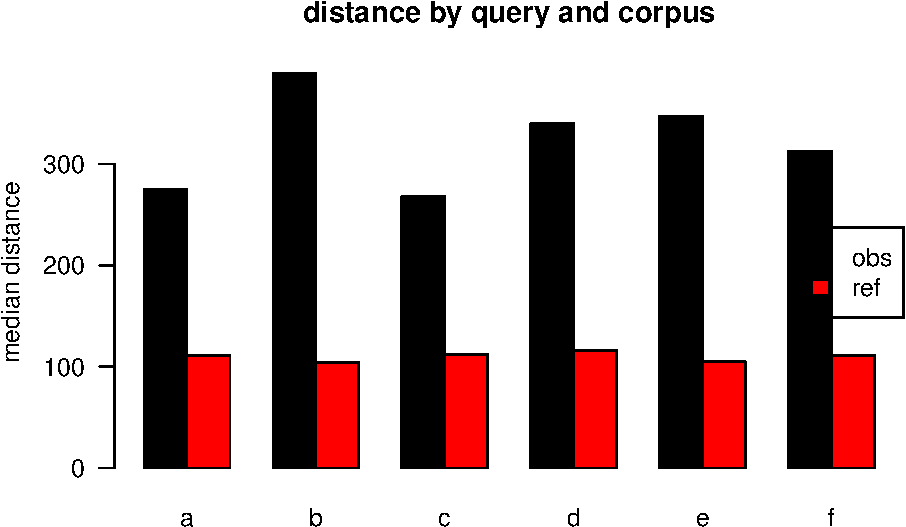
\includegraphics{spund-pub_files/figure-latex/barplot-median4-1} \caption{median distances over query/corpus, normalised to ref, distance ceiling =  outliers removed}\label{fig:barplot-median4}
\end{figure}

\begin{figure}[H]
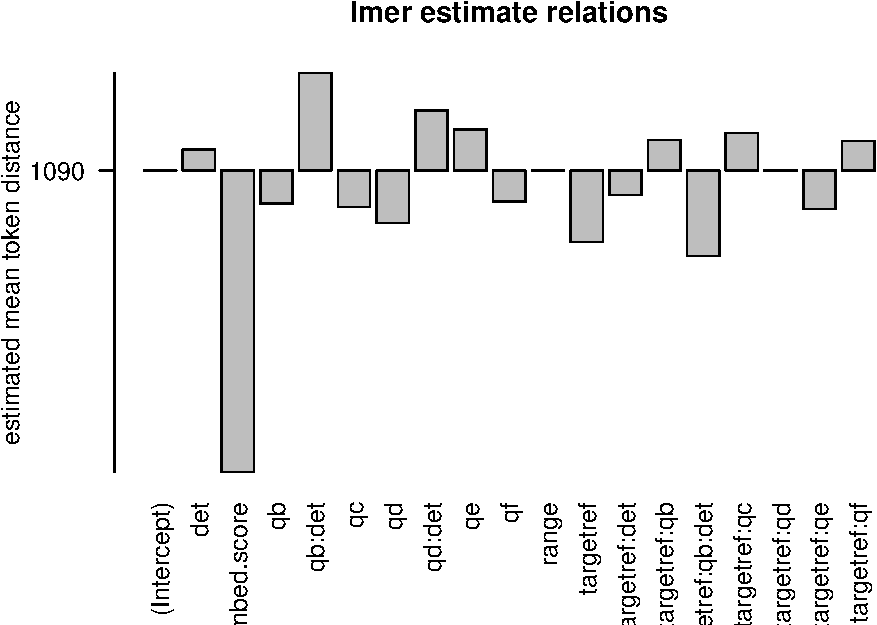
\includegraphics{spund-pub_files/figure-latex/lmeplot4-1} \caption{distances relation, normalised to ref, distance ceiling =  outliers removed}\label{fig:lmeplot4}
\end{figure}

\begin{figure}[H]
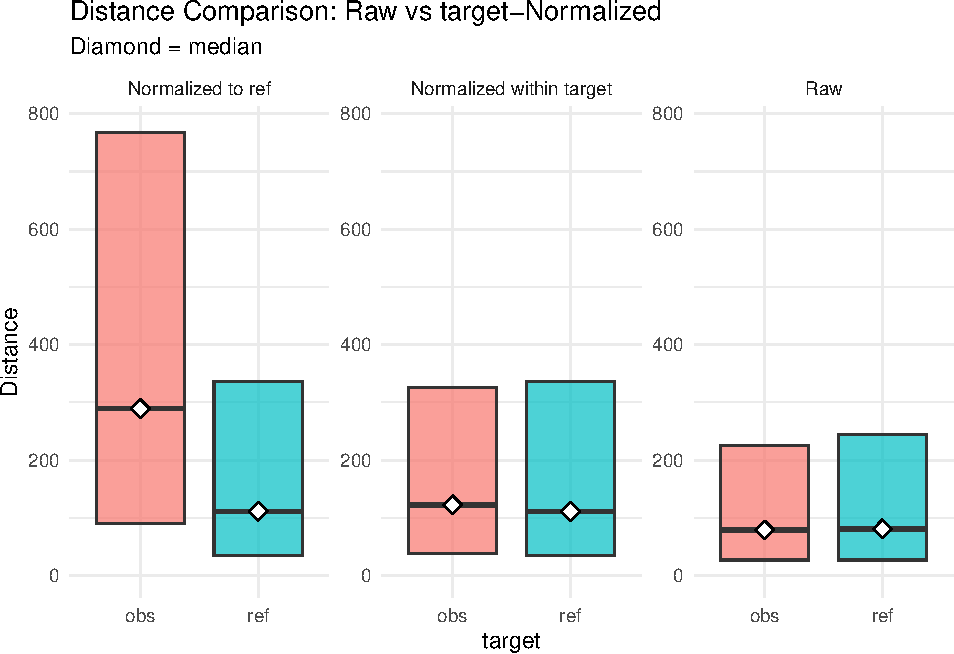
\includegraphics{spund-pub_files/figure-latex/gplot4-1} \caption{distances normalised vs. raw}\label{fig:gplot4}
\end{figure}

\section{evaluation model: 6}\label{evaluation-model-6}

\subsection{meta}\label{meta-4}

eval output data: 13, not normalised, distance ceiling =outliers removed

\subsection{parameter setting}\label{parameter-setting-4}

\begin{verbatim}
##             value
## norm_target      
## det.t        TRUE
## limit        TRUE
## author       TRUE
## url          TRUE
## embed1       TRUE
## embed2          f
## range1       TRUE
## range2          f
## rel         FALSE
## lme         FALSE
## lemma       FALSE
\end{verbatim}

\subsection{anova analysis}\label{anova-analysis-4}

\subsubsection{anova plain}\label{anova-plain-4}

formula: {[}\texttt{dist\ \textasciitilde{}\ target*q*det}{]}

\begin{verbatim}
##                  Df     Sum Sq Mean Sq F value    Pr(>F)    
## target            1    3284330 3284330 84.1223 < 2.2e-16 ***
## q                 5    1633205  326641  8.3663  6.39e-08 ***
## det               1     431404  431404 11.0496 0.0008873 ***
## target:q          5     441118   88224  2.2597 0.0457798 *  
## target:det        1      16732   16732  0.4286 0.5126999    
## q:det             2      25549   12774  0.3272 0.7209470    
## target:q:det      1       6009    6009  0.1539 0.6948226    
## Residuals    126209 4927490433   39042                      
## ---
## Signif. codes:  0 '***' 0.001 '**' 0.01 '*' 0.05 '.' 0.1 ' ' 1
\end{verbatim}

\subsubsection{anova of linear regression model}\label{anova-of-linear-regression-model-4}

{[}\texttt{anova(summary(lmer))}{]}

\begin{verbatim}
## Type III Analysis of Variance Table with Satterthwaite's method
##                Sum Sq  Mean Sq NumDF  DenDF   F value Pr(>F)    
## target            218      218     1  17034    0.0061 0.9377    
## q              109358    21872     5 124317    0.6129 0.6901    
## det             20678    20678     1 121247    0.5794 0.4465    
## range        15332432 15332432     1    912  429.6377 <2e-16 ***
## embed.score  77286239 77286239     1 105351 2165.6761 <2e-16 ***
## target:q       304923    60985     5 125126    1.7089 0.1287    
## target:det      17833    17833     1 124982    0.4997 0.4796    
## q:det           37151    18576     2 123066    0.5205 0.5942    
## target:q:det    23985    23985     1 124972    0.6721 0.4123    
## ---
## Signif. codes:  0 '***' 0.001 '**' 0.01 '*' 0.05 '.' 0.1 ' ' 1
\end{verbatim}

\subsubsection{linear regression coefficients}\label{linear-regression-coefficients-4}

formula: {[}\texttt{dist\ \textasciitilde{}\ target*q*det+(1\textbar{}aut\_id)+range+(embed.score)+(1\textbar{}url\_id)}{]}

\begin{verbatim}
## Linear mixed model fit by REML. t-tests use Satterthwaite's method [
## lmerModLmerTest]
## Formula: eval(expr(lmeform))
##    Data: dfa
## 
## REML criterion at convergence: 1685333
## 
## Scaled residuals: 
##     Min      1Q  Median      3Q     Max 
## -2.0402 -0.6622 -0.3317  0.3419  4.1697 
## 
## Random effects:
##  Groups   Name        Variance Std.Dev.
##  aut_id   (Intercept)  1394     37.34  
##  url_id   (Intercept)  1072     32.74  
##  Residual             35687    188.91  
## Number of obs: 126226, groups:  aut_id, 8238; url_id, 2145
## 
## Fixed effects:
##                    Estimate Std. Error         df t value Pr(>|t|)    
## (Intercept)       2.533e+02  3.618e+00  1.966e+04  70.000  < 2e-16 ***
## targetref         1.326e+00  2.954e+00  1.890e+03   0.449  0.65362    
## qb               -8.195e+00  1.300e+01  1.239e+05  -0.630  0.52845    
## qc               -8.144e+00  4.675e+00  1.243e+05  -1.742  0.08150 .  
## qd               -1.117e+02  1.902e+02  1.212e+05  -0.587  0.55726    
## qe                1.392e+01  3.248e+00  1.256e+05   4.285 1.83e-05 ***
## qf               -6.628e+00  4.145e+00  1.253e+05  -1.599  0.10981    
## det               3.793e+00  4.058e+00  1.245e+05   0.935  0.35005    
## range             1.535e-02  7.406e-04  9.124e+02  20.728  < 2e-16 ***
## embed.score      -3.110e+02  6.682e+00  1.054e+05 -46.537  < 2e-16 ***
## targetref:qb      4.017e+00  1.464e+01  1.244e+05   0.274  0.78373    
## targetref:qc      4.577e+00  1.089e+01  1.253e+05   0.420  0.67442    
## targetref:qd     -2.061e+00  1.069e+01  1.253e+05  -0.193  0.84707    
## targetref:qe     -2.134e+01  8.099e+00  1.255e+05  -2.635  0.00841 ** 
## targetref:qf      8.889e+00  1.031e+01  1.254e+05   0.862  0.38849    
## targetref:det     1.178e+00  9.236e+00  1.253e+05   0.127  0.89855    
## qb:det            1.714e+01  1.428e+01  1.239e+05   1.200  0.23002    
## qd:det            1.126e+02  1.902e+02  1.212e+05   0.592  0.55380    
## targetref:qb:det -1.710e+01  2.086e+01  1.250e+05  -0.820  0.41233    
## ---
## Signif. codes:  0 '***' 0.001 '**' 0.01 '*' 0.05 '.' 0.1 ' ' 1
## fit warnings:
## fixed-effect model matrix is rank deficient so dropping 7 columns / coefficients
## Some predictor variables are on very different scales: consider rescaling
\end{verbatim}

\subsection{plots}\label{plots-4}

\begin{figure}[H]
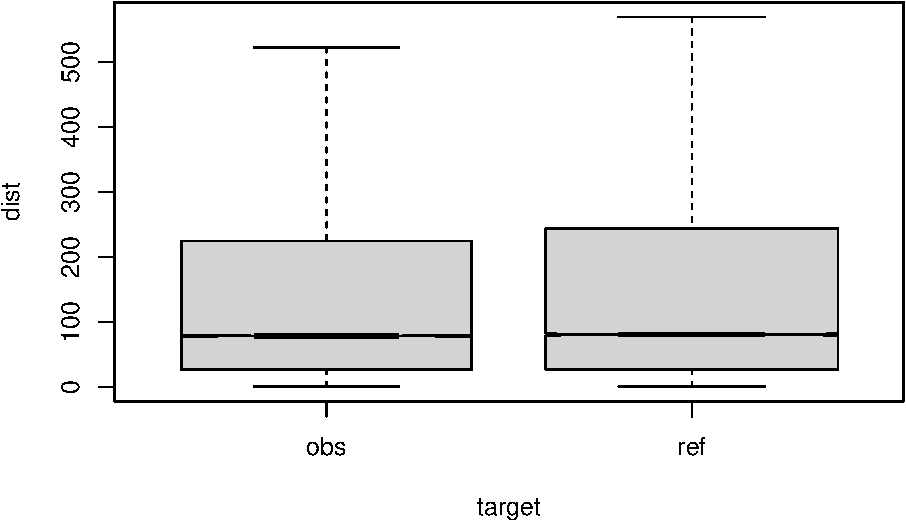
\includegraphics{spund-pub_files/figure-latex/boxplot16-1} \caption{compare distances by corpus, not normalised, distance ceiling =outliers removed}\label{fig:boxplot16}
\end{figure}

\begin{figure}[H]
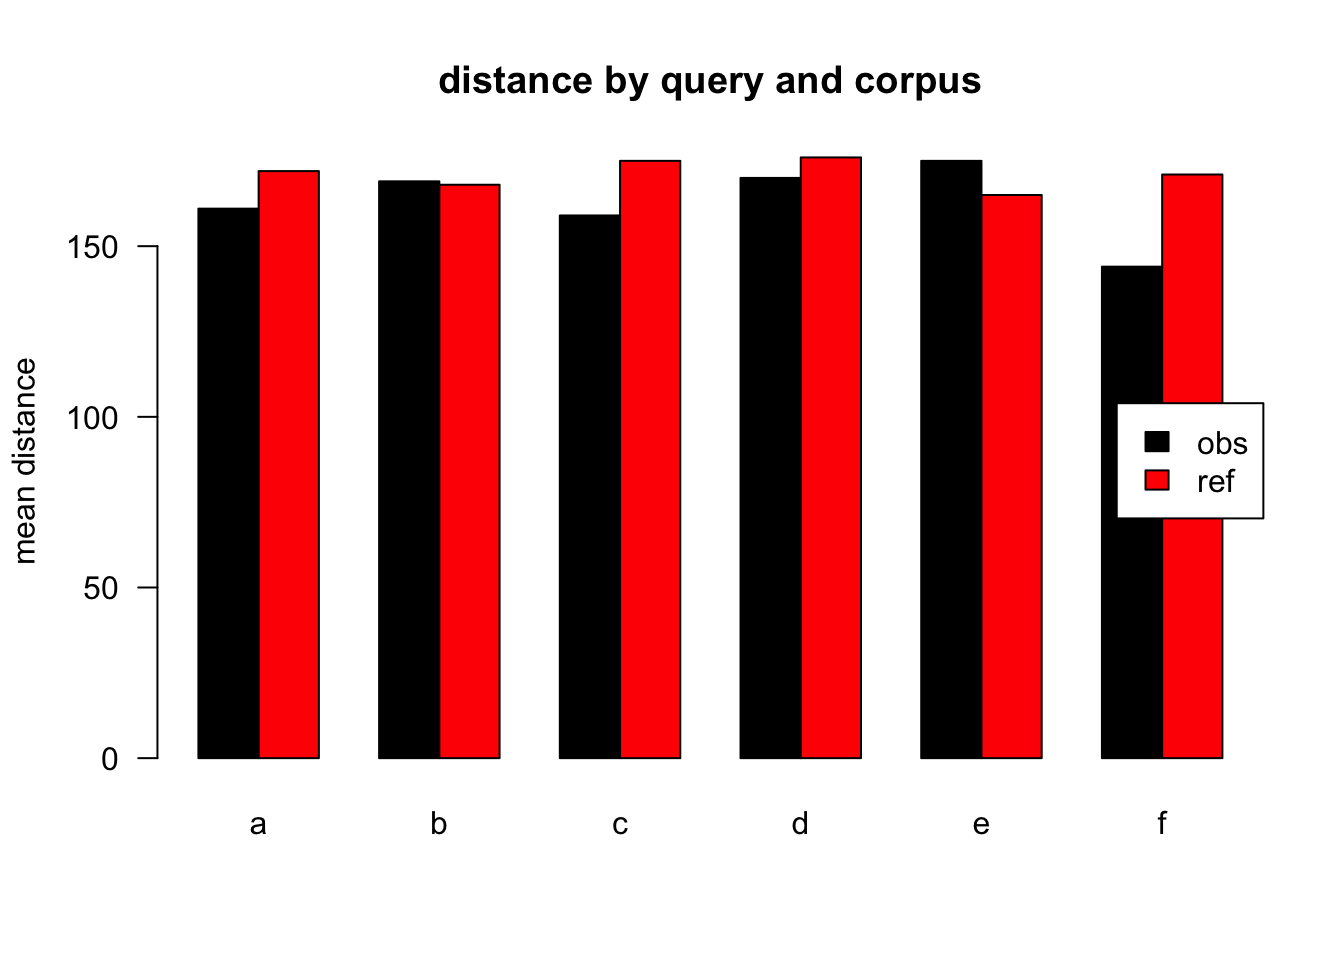
\includegraphics{spund-pub_files/figure-latex/barplot-mean6-1} \caption{mean distances over query/corpus, not normalised, distance ceiling =outliers removed}\label{fig:barplot-mean6}
\end{figure}

\begin{longtable}[]{@{}llrrr@{}}
\caption{\label{tab:dfe-table6}mean/median table for model: 6}\tabularnewline
\toprule\noalign{}
target & q & n & mean & median \\
\midrule\noalign{}
\endfirsthead
\toprule\noalign{}
target & q & n & mean & median \\
\midrule\noalign{}
\endhead
\bottomrule\noalign{}
\endlastfoot
obs & a & 42836 & 161 & 77 \\
ref & a & 58615 & 172 & 81 \\
obs & b & 2116 & 169 & 109 \\
ref & b & 1130 & 168 & 78 \\
obs & c & 5770 & 159 & 75 \\
ref & c & 1274 & 175 & 84 \\
obs & d & 5654 & 170 & 86 \\
ref & d & 1525 & 176 & 83 \\
obs & e & 3911 & 175 & 92 \\
ref & e & 671 & 165 & 71 \\
obs & f & 2311 & 144 & 62 \\
ref & f & 413 & 171 & 82 \\
\end{longtable}

\begin{figure}[H]
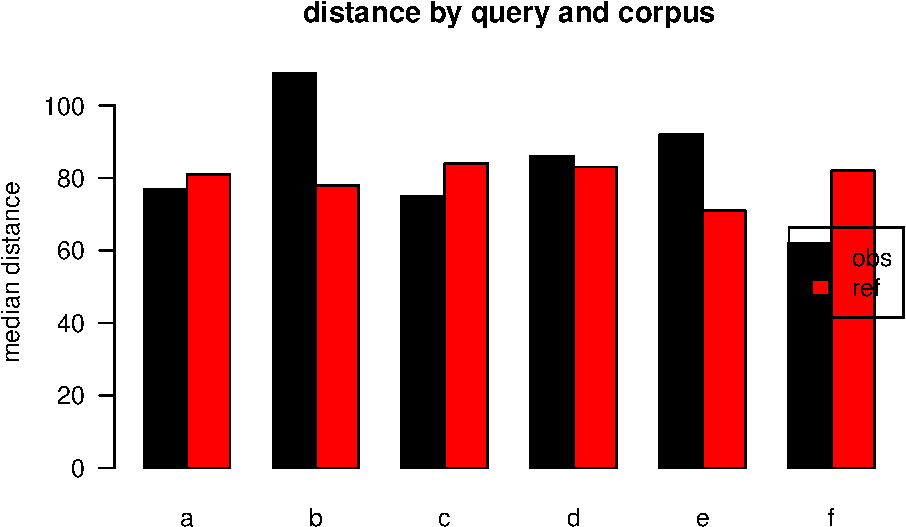
\includegraphics{spund-pub_files/figure-latex/barplot-median6-1} \caption{median distances over query/corpus, not normalised, distance ceiling =outliers removed}\label{fig:barplot-median6}
\end{figure}

\begin{figure}[H]
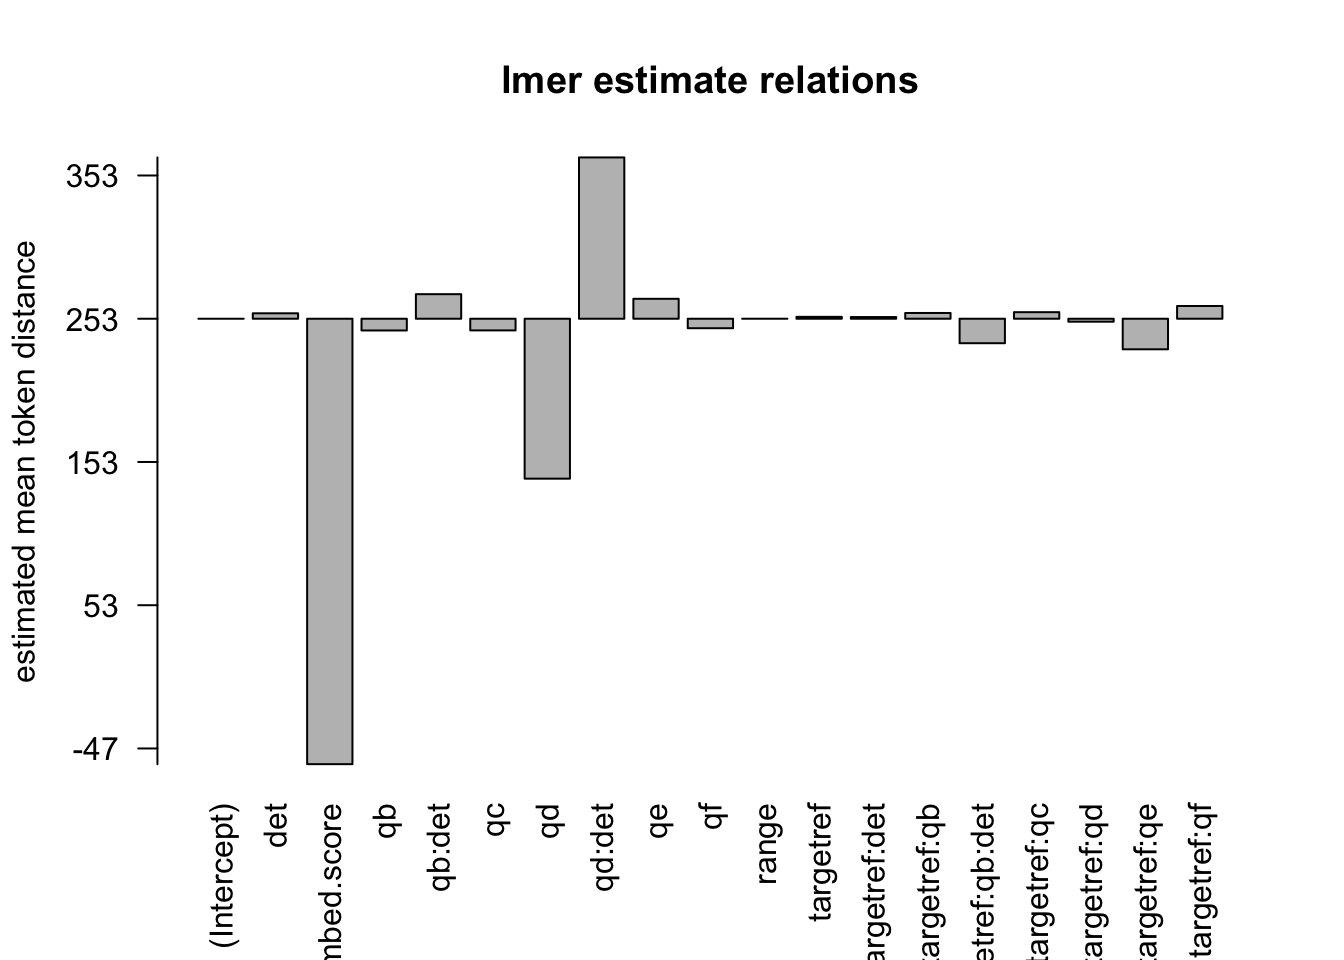
\includegraphics{spund-pub_files/figure-latex/lmeplot6-1} \caption{distances relation, not normalised, distance ceiling =outliers removed}\label{fig:lmeplot6}
\end{figure}

\begin{figure}[H]
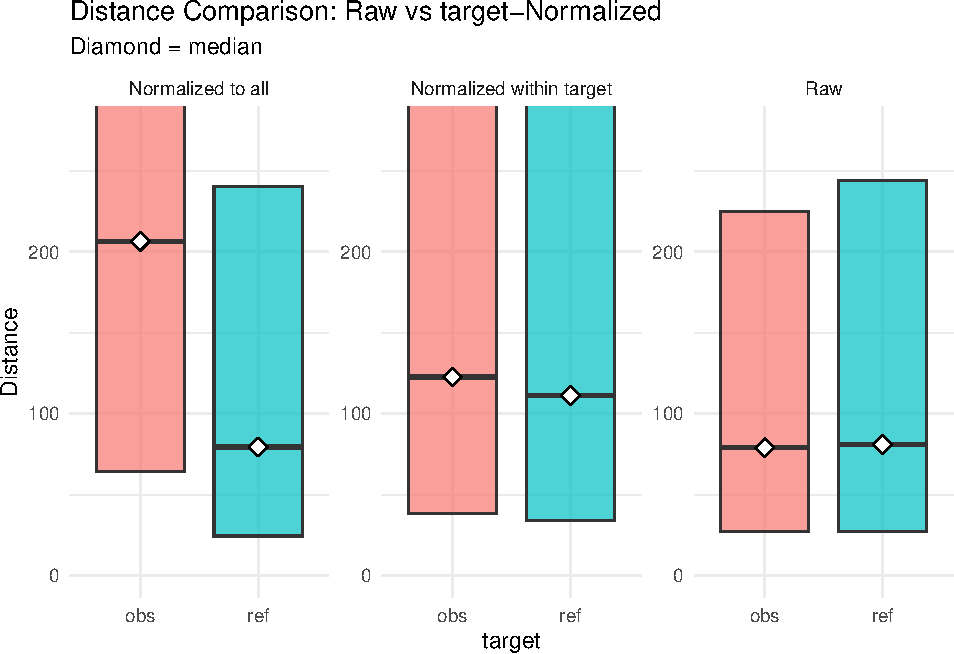
\includegraphics{spund-pub_files/figure-latex/gplot6-1} \caption{distances normalised vs. raw}\label{fig:gplot6}
\end{figure}

\section{Selbständigkeit: benutzte Hilfestellung}\label{selbstuxe4ndigkeit-benutzte-hilfestellung}

In der vorliegenden Arbeit wurden keinerlei nicht erlaubte Hilfsmittel zur Erstellung von Inhalten verwendet. Die Benutzung von KI beschränkt sich auf (Tabelle):

\begin{table}

\caption{\label{tab:kitable}verwendete Hilfsmittel}
\resizebox{\ifdim\width>\linewidth\linewidth\else\width\fi}{!}{
\begin{tabular}[t]{ll}
\toprule
Hilfsmittel & Verwendung\\
\midrule
github copilot & Hilfe bei der Skripterstellung (R, Python) zur 
Programmierung der Distanzenberechnung, semantic embeddings und statistischen Auswertung\\
chatgpt.com & dito\\
claude.ai & dito\\
deepseek.com & dito\\
nomic-embed-text (model) & calculate semantic embeddings\\
\bottomrule
\end{tabular}}
\end{table}

\begin{center}\rule{0.5\linewidth}{0.5pt}\end{center}

\section{references}\label{references}

literature used and alii\ldots{}

\phantomsection\label{refs}
\begin{CSLReferences}{1}{0}
\bibitem[\citeproctext]{ref-bates_fitting_2015}
Bates, Douglas, Martin Mächler, Ben Bolker, and Steve Walker. 2015. {``Fitting {Linear} {Mixed}-{Effects} {Models} {Using} Lme4.''} \emph{Journal of Statistical Software} 67 (1): 1--48. \url{https://doi.org/10.18637/jss.v067.i01}.

\bibitem[\citeproctext]{ref-de_marneffe_universal_2021}
De Marneffe, Marie-Catherine, Christopher D. Manning, Joakim Nivre, and Daniel Zeman. 2021. {``Universal {Dependencies}.''} \emph{Computational Linguistics}, May, 1--54. \url{https://doi.org/10.1162/coli_a_00402}.

\bibitem[\citeproctext]{ref-huggingface_all-minilm-l6-v2_2025}
HuggingFace. 2025. {``All-{MiniLM}-{L6}-V2 · {Hugging} {Face}.''} \emph{Sentence Transformers}. \url{https://huggingface.co/sentence-transformers/all-MiniLM-L6-v2}.

\bibitem[\citeproctext]{ref-kjell_text-package_2023}
Kjell, Oscar, Salvatore Giorgi, and H. Andrew Schwartz. 2023. {``The Text-Package: {An} {R}-Package for {Analyzing} and {Visualizing} {Human} {Language} {Using} {Natural} {Language} {Processing} and {Deep} {Learning}.''} \emph{Psychological Methods}. \url{https://doi.org/10.1037/met0000542}.

\bibitem[\citeproctext]{ref-kuperberg_language_2010}
Kuperberg, Gina R. 2010. {``Language in Schizophrenia {Part} 2: {What} Can Psycholinguistics Bring to the Study of Schizophrenia\ldots and Vice Versa?''} \emph{Language and Linguistics Compass} 4 (8): 590--604. \url{https://doi.org/10.1111/j.1749-818X.2010.00217.x}.

\bibitem[\citeproctext]{ref-lee_higher-order_2018}
Lee, Kenton, Luheng He, and Luke Zettlemoyer. 2018. {``Higher-Order {Coreference} {Resolution} with {Coarse}-to-Fine {Inference}.''} arXiv. \url{https://doi.org/10.48550/arXiv.1804.05392}.

\bibitem[\citeproctext]{ref-mishara_klaus_2010}
Mishara, Aaron L. 2010. {``Klaus {Conrad} (1905--1961): {Delusional} {Mood}, {Psychosis}, and {Beginning} {Schizophrenia}.''} \emph{Schizophrenia Bulletin} 36 (1): 9--13. \url{https://doi.org/10.1093/schbul/sbp144}.

\bibitem[\citeproctext]{ref-noauthor_nomic-ainomic-embed-text-v15_2024}
{``Nomic-Ai/Nomic-Embed-Text-V1.5 · {Hugging} {Face}.''} 2024. \url{https://huggingface.co/nomic-ai/nomic-embed-text-v1.5}.

\bibitem[\citeproctext]{ref-noauthor_nomic-embed-text_nodate}
{``Nomic-Embed-Text.''} n.d. Accessed October 6, 2025. \url{https://ollama.com/nomic-embed-text}.

\bibitem[\citeproctext]{ref-nussbaum_nomic_2024}
Nussbaum, Zach, John X. Morris, Brandon Duderstadt, and Andriy Mulyar. 2024. {``Nomic {Embed}: {Training} a {Reproducible} {Long} {Context} {Text} {Embedder}.''} \url{https://huggingface.co/nomic-ai/nomic-embed-text-v1.5}.

\bibitem[\citeproctext]{ref-ottiram_ottirammmax2_2025}
ottiram. 2025. {``Ottiram/{MMAX2}.''} \url{https://github.com/ottiram/MMAX2}.

\bibitem[\citeproctext]{ref-poesio_massimo_arrau_2013}
Poesio, Massimo, Artstein, Ron, Uryupina, Olga, Rodriguez, Kepa, Delogu, Francesca, Bristot, Antonella, and Hitzeman, Janet. 2013. {``The {ARRAU} {Corpus} of {Anaphoric} {Information}.''} Linguistic Data Consortium. \url{https://doi.org/10.35111/Y3MR-HE10}.

\bibitem[\citeproctext]{ref-prince_toward_1981}
Prince, Ellen F. 1981. {``Toward a Taxonomy of Given-New Information.''} In \emph{Syntax and Semantics: {Vol}. 14. {Radical} {Pragmatics}}, edited by P. Cole, 223--55. New York: Academic Press.

\bibitem[\citeproctext]{ref-rivera_redditextractor_2023}
Rivera, Ivan. 2023. {``{RedditExtractoR}: {Reddit} {Data} {Extraction} {Toolkit}.''} \url{https://CRAN.R-project.org/package=RedditExtractoR}.

\bibitem[\citeproctext]{ref-schwarz_poster_2025}
Schwarz, St. 2025. {``Poster Appendix: This Papers Scripts for Corpus Build and Statistics on Github.''} \url{https://github.com/esteeschwarz/SPUND-LX/tree/main/psych/HA}.

\bibitem[\citeproctext]{ref-wijffels_udpipe_2023}
Wijffels, Jan. 2023. \emph{Udpipe: {Tokenization}, {Parts} of {Speech} {Tagging}, {Lemmatization} and {Dependency} {Parsing} with the '{UDPipe}' '{NLP}' {Toolkit}}. \url{https://CRAN.R-project.org/package=udpipe}.

\bibitem[\citeproctext]{ref-zimmerer_deictic_2017}
Zimmerer, Vitor C., Stuart Watson, Douglas Turkington, I. Nicol Ferrier, and Wolfram Hinzen. 2017. {``Deictic and {Propositional} {Meaning}---{New} {Perspectives} on {Language} in {Schizophrenia}.''} \emph{Frontiers in Psychiatry} 8 (February). \url{https://doi.org/10.3389/fpsyt.2017.00017}.

\end{CSLReferences}

\end{document}
